\documentclass{report_template_oxford}

\title{3YP Report}
\subtitle{Multiagent Autonomous Drone System for Landmine Detection}
\author{Group B: Huirui Dai, Samuel Grace, Rory Millard, Jihwan Shin, Thomas Turner}
\date{March 2025}

\begin{document}
\maketitle

% Abstract
% - Concise summary of report
% - Naming of essential outcomes
% - As short as possible while providing key points
% - Less than 1 page
\pagenumbering{roman}
\newpage
\addcontentsline{toc}{section}{Abstract}
\fancyhead[C]{Student author of section}
\section*{Abstract}

Add abstract here.

\newpage
\fancyhead[C]{}
\tableofcontents

\newpage
\addcontentsline{toc}{section}{List of Figures}
\listoffigures

\newpage
\addcontentsline{toc}{section}{List of Tables}
\listoftables

\newpage
\addcontentsline{toc}{section}{Glossary}
\printglossaries

\newpage
\pagenumbering{arabic}
\fancyhead[C]{Student}
\section{Introduction} \label{introduction}

\fancyhead[C]{Student}
\subsection{Sub-Introduction}

\newacronym{UAV}{UAV}{Unmanned Aerial Vehicle}
\newacronym{SPI}{SPI}{Serial Peripheral Interface}
\newacronym{CAN}{CAN}{Controller Area Network}
\newacronym{UART}{UART}{Universal Asynchronous Receiver / Transmitter}
\newacronym{IMU}{IMU}{Inertial Measurement Unit}
\newacronym{ESC}{ESC}{Electronic Speed Controller}
\newacronym{RPM}{RPM}{Rotations Per Minute}

\newpage
\pagenumbering{arabic}
\fancyhead[C]{Jihwan Shin}
\section{Mission Planning} \label{missionplanning}

In \gls{cpp} we must cover the entire region of interest \cite{cabreira2019cpp}. As mentioned in section~\ref{hardware}, we will use thermal and GPSAR sensors.

\newpage
\pagenumbering{arabic}
\fancyhead[C]{Huirui Dai}
\section{Hardware} \label{hardware}

\newpage
\fancyhead[C]{Huirui Dai}
\setlength{\parindent}{0pt}

\section{Data Acquisition} \label{data acquisition}

\subsection{Landmines}

The selection of sensing hardware in our multi-drone landmine detection system relies on a clear understanding of the target: landmines. Landmines differ widely in size, materials, triggering mechanisms, and intended targets. These physical differences strongly affect how detectable they are, especially when using drones with limited payload capacity. This section outlines the main landmine types and highlights the features that influence detection. This overview supports informed decisions on sensor selection and data acquisition in our system.

Landmines are commonly classified into two main categories based on their intended targets: anti-tank landmines (ATLs) and anti-personnel landmines (APLs).
\footnote{\url{https://en.wikipedia.org/wiki/Land_mine}}

ATLs are designed to disable or destroy heavy vehicles such as tanks or armored transports. They are typically large, with diameters ranging from 13 to 40 cm, and contain 6 to 11 kg of explosives\cite{paik2002image}. These mines are generally triggered by high pressures and are often buried beneath roadways or terrain. Traditional ATLs use metal casings, but modern designs may incorporate plastic or composite materials to reduce detectability \cite{evans2024detection}. Based on their activation mechanisms, ATLs can be classified into pressure-activated blast mines, tilt-rod or magnetic mines, and side-attack mines.

APLs are intended to injure or kill individuals on foot. They are much smaller than ATLs, typically ranging from 6 to 15 cm in diameter, and contain only 0.1 to 4 kg of explosives\cite{paik2002image}. These mines are triggered by very low pressure, often below 10 kg, which makes them highly dangerous and difficult to detect. APLs are commonly constructed from plastic, rubber, or other low-metal-content materials, further reducing their detectability \cite{kaya2017buried}. Like ATLs, APLs are also divided into subtypes, including blasting mines, bounding fragmentation mines, and directional fragmentation mines.

\begin{figure}[h]
    \centering
    \begin{subfigure}[b]{0.24\textwidth}
        \centering
        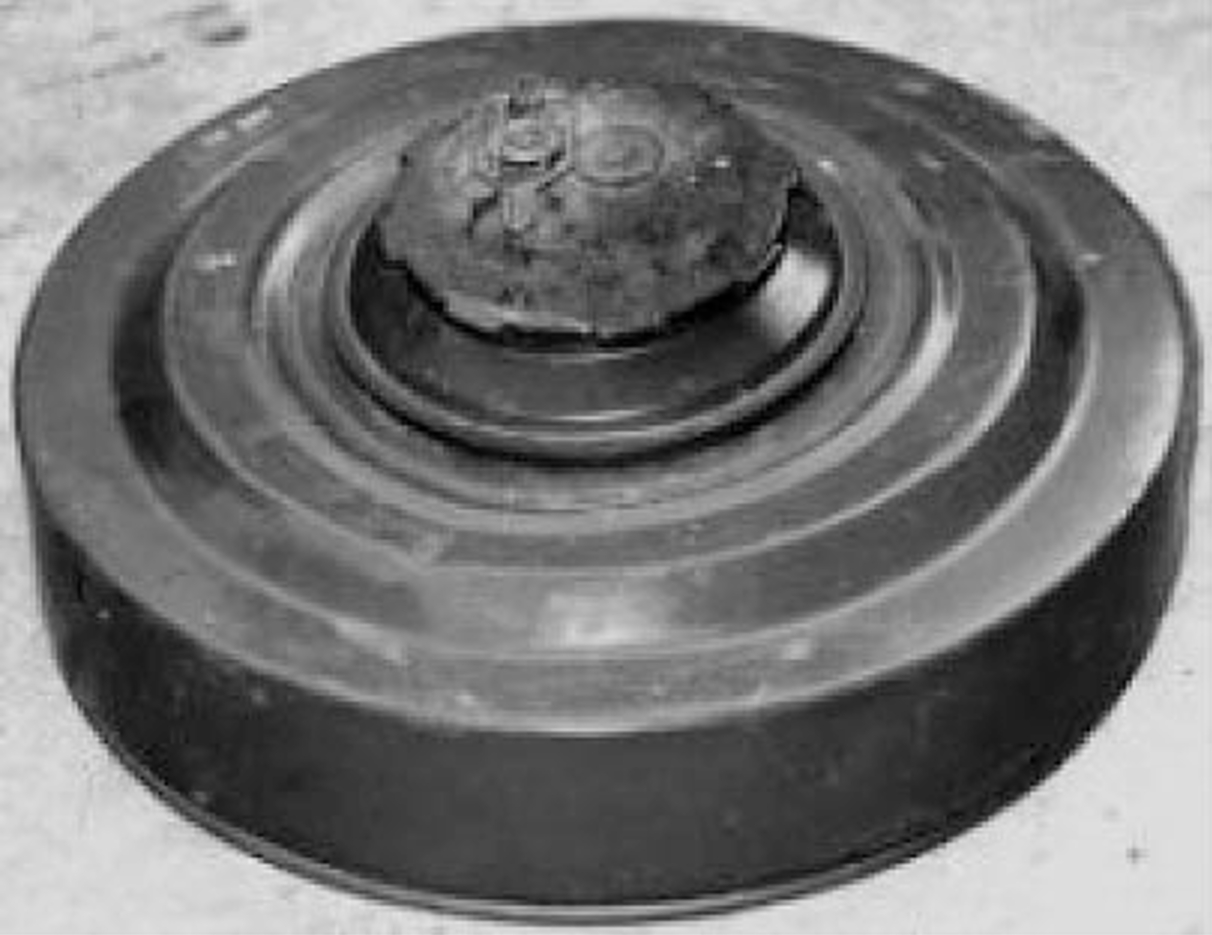
\includegraphics[height=2cm]{figs/Huirui/tm62m.png}
        \subcaption*{(a)}
    \end{subfigure}
    \begin{subfigure}[b]{0.24\textwidth}
        \centering
        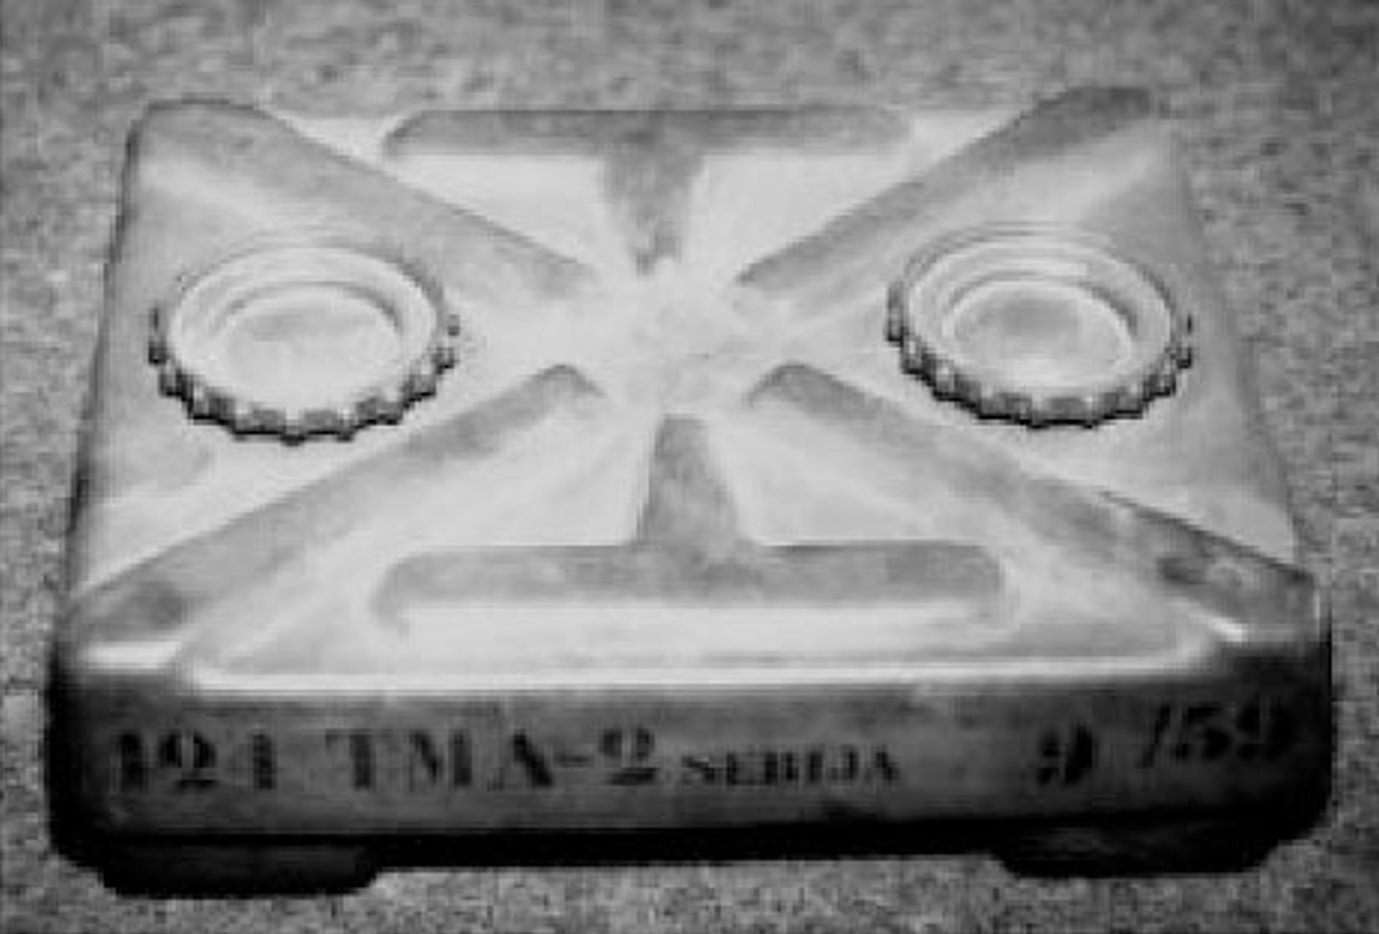
\includegraphics[height=2cm]{figs/Huirui/tma2.png}
        \subcaption*{(b)}
    \end{subfigure}
    \begin{subfigure}[b]{0.24\textwidth}
        \centering
        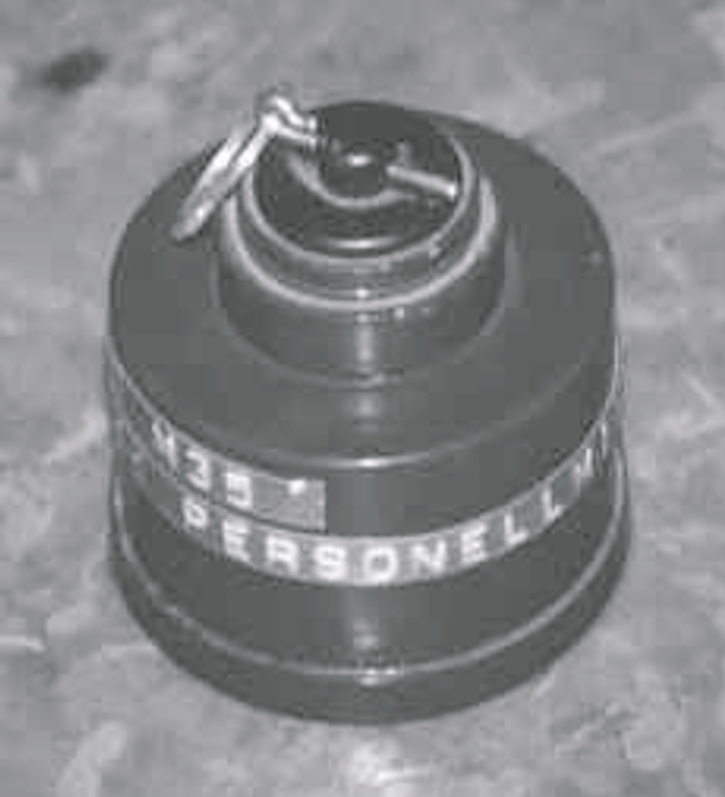
\includegraphics[height=2cm]{figs/Huirui/prbm35.png}
        \subcaption*{(c)}
    \end{subfigure}
    \begin{subfigure}[b]{0.24\textwidth}
        \centering
        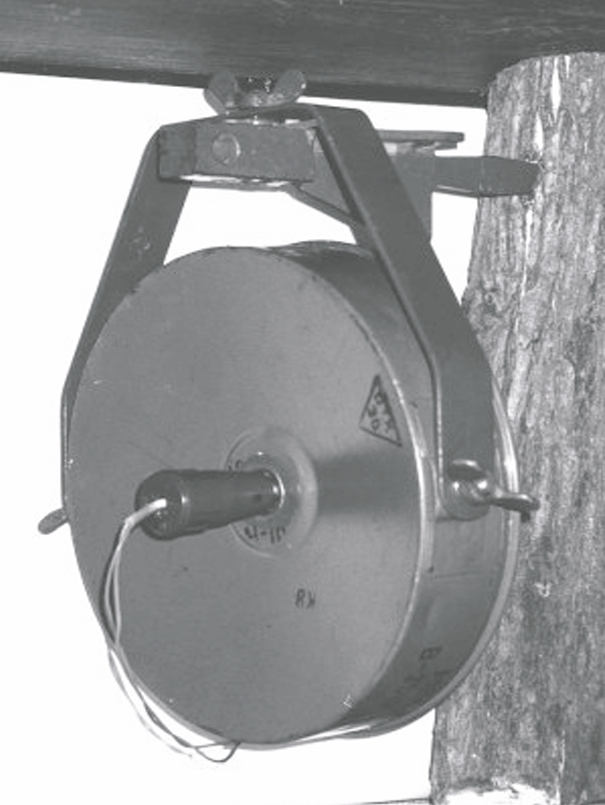
\includegraphics[height=2cm]{figs/Huirui/mon100.png}
        \subcaption*{(d)}
    \end{subfigure}

    \caption{Typical ATLs and APLs: (a) TM-62M, (b) TMA-2, (c) PRB-M35, and (d) MON-100~\cite{paik2002image}.}
    \label{fig:mine_examples}
\end{figure}


\begin{table}[h]
    \centering
    \small
    \renewcommand{\arraystretch}{1.3}
    \caption{Specifications for selected ATLs and APLs~\cite{paik2002image}.}
    \label{tab:mine_specs}
    \begin{tabular}{l p{2.8cm} p{2.8cm} p{2.8cm} p{2.8cm}}
        \toprule
        \textbf{Model No.} & \textbf{TM-62M} & \textbf{TMA-2} & \textbf{PRB-M35} & \textbf{MON-100} \\
        \midrule
        Type & ATL & ATL & APL & APL \\
        Height (cm) & 11.2 & 14.0 & 5.7 & 8.2 \\
        Diameter / Width (cm) & 31.6 & 26.0 × 20.0 & 6.4 & 23.6 \\
        Weight (kg) & 8.5 & 7.5 & 0.16 & 5.0 \\
        Material & Steel & Plastic & Plastic & Steel \\
        Sensitivity & 200 kg & 120 kg & 8 kg & Depends on fuses \\
        \bottomrule
    \end{tabular}
\end{table}

Figure~\ref{fig:mine_examples} shows four representative examples of ATLs and APLs, and Table~\ref{tab:mine_specs} summarizes their key structural specifications. As the table indicates, both ATLs and APLs can be constructed from metallic, low-metallic, or non-metallic materials. However, APLs are significantly smaller in size, which make them more difficult to detect, especially from aerial platforms. And from a technical perspective, a system capable of reliably detecting small APLs is also likely to detect the larger ATLs. Also, nowadays APLs are more responsible for the vast majority of civilian injuries and deaths in post-conflict areas compared with ATLs \cite{unmas2021handbook}, which underscores their humanitarian significance. For these reasons, our project focuses on the detection of anti-personnel landmines.

\subsection{Sensors}

\subsubsection{Landmine Detection Techniques}

Landmine detection technologies have evolved to encompass a wide range of sensing principles, each targeting specific physical, chemical, or biological characteristics of surface-laid and buried mines. Broadly, these methods can be categorized into five general classes: \textit{\textbf{electromagnetic induction-based} techniques}, \textit{\textbf{radiowave and microwave-based} systems}, \textit{\textbf{mechanical and vibro-acoustic} methods}, \textit{\textbf{spectral and thermal imaging} approaches}, and \textit{\textbf{chemical and biological} sensing methods}. Within each class, a variety of specialized detection technologies have been developed, including traditional metal detectors, ground-penetrating radar, infrared and hyperspectral imaging, seismic/acoustic sensors, vapor detection, and biosensors. Each of these approaches offers distinct advantages and faces specific limitations, especially when adapted to drone-based platforms for remote and efficient minefield scanning. In the following subsections, each class is explored in detail, with emphasis on the operating principles, detection capabilities, challenges, and documented UAV-based applications.

\paragraph{Electromagnetic Induction-Based Techniques}

Electromagnetic induction (EMI) methods operate by exploiting the interaction between electromagnetic fields and conductive or magnetic materials in the ground. These systems are typically composed of a transmitter coil that emits a time-varying electromagnetic field into the soil. When this field encounters a conductive object—such as a landmine with metallic components—it induces eddy currents within the object, which in turn generate a secondary magnetic field. This field is detected by a receiver coil, and the resulting signal is processed to infer the presence of the object. These principles form the basis of conventional \textbf{metal detectors}~\cite{gichd2006guidebook}.

In contrast, \textbf{magnetic sensors} or magnetometers do not actively induce eddy currents but instead measure disturbances in the Earth's ambient magnetic field caused by nearby ferromagnetic objects. While metal detectors rely on electromagnetic induction to detect a wide range of conductive materials, magnetometers are primarily sensitive to ferrous (iron-containing) materials and are particularly effective in detecting anomalies in the magnetic environment\footnote{\label{magnetometerfootnote}\url{https://www.sphengineering.com/integrated-systems/technologies/magnetometer}}.

Several specialized EMI sensors have been developed, including induction coil imaging systems that generate spatial maps of subsurface metallic objects, conductivity meters that monitor variations in soil conductivity through eddy current decay, and a range of magnetometers such as fluxgate, proton precession, optically pumped atomic, and meandering winding designs. Each sensor type offers specific trade-offs in sensitivity, resolution, and robustness, and may be selected based on the expected mine characteristics and deployment constraints~\cite{Gooneratne2004ARO, Bruschini1997ASO}.

\textbf{Strengths:} Electromagnetic induction (EMI) methods are among the most mature and widely adopted landmine detection techniques. They are well-established, commercially available, and commonly implemented in handheld and vehicle-mounted systems~\cite{gichd2006guidebook}. These methods are particularly effective for detecting the vast majority of deployed landmines that contain some amount of metal, including minimum-metal mines where metallic elements are limited to components such as detonator capsules or striker pins~\cite{gichd2006guidebook}. With appropriately sized coil systems, EMI devices can achieve considerable depth penetration—for example, up to 70 cm for unexploded ordnance (UXO) and metallic mines~\cite{gichd2006guidebook}. Magnetic sensors, in particular, are versatile and have been applied beyond demining, including the detection of buried utilities, iron ore deposits, archaeological artifacts, and submarines due to their sensitivity to ferrous materials\textsuperscript{\ref{magnetometerfootnote}}.

\textbf{Limitations:} Despite their widespread use, EMI-based methods have significant limitations. A key drawback is their inability to distinguish between landmines and other metallic objects, often leading to very high false alarm rates—ranging from 100 to 1000 false detections per real mine in cluttered environments~\cite{Bruschini1997ASO, robledo2009survey}. Their effectiveness decreases significantly when detecting modern plastic-cased or low-metal-content mines, which often contain only a few grams of metal~\cite{gichd2006guidebook}. These sensors are also susceptible to interference from magnetic or conductive soils, such as laterite-rich ground or coastal sands, and their performance deteriorates in the presence of electromagnetic noise from power lines and nearby electronics~\cite{gichd2006guidebook}. Additionally, footprint size reduces with depth, and passive magnetometers may fail to detect certain non-ferrous materials, such as gold or copper, which do not significantly alter the ambient magnetic field\textsuperscript{\ref{magnetometerfootnote}}.

\textbf{Drone-Based Applications:} EMI sensors have been successfully integrated into UAV platforms in numerous studies~\cite{yoo2020drone,7529819,mu2020automatic,yoo2021application,BARNAWI2022441,rs15153813,barnawi2023graph,Barnawi2023ADL,s21093175,9251007,Safatly04032021,10745471,Stankevich2024OpticalAM,Joo2022OptimizationDM,rs16162916,Yoo2024UnmannedAV,rs16244732,Poliachenko_Kozak_Bakhmutov_Cherkes_Bilyi_2025}. These include implementations of both lightweight metal detectors and magnetic sensors for aerial surveying of minefields. Figure~\ref{fig:metal_detector_drone} shows an example of a UAV equipped with a metal detector for low-altitude scanning, while Figure~\ref{fig:magnetometer_drone} illustrates a UAV-mounted magnetometer designed for aerial magnetic anomaly detection. 

\begin{figure}[h!]
    \centering
    \begin{subfigure}[b]{0.48\linewidth}
        \centering
        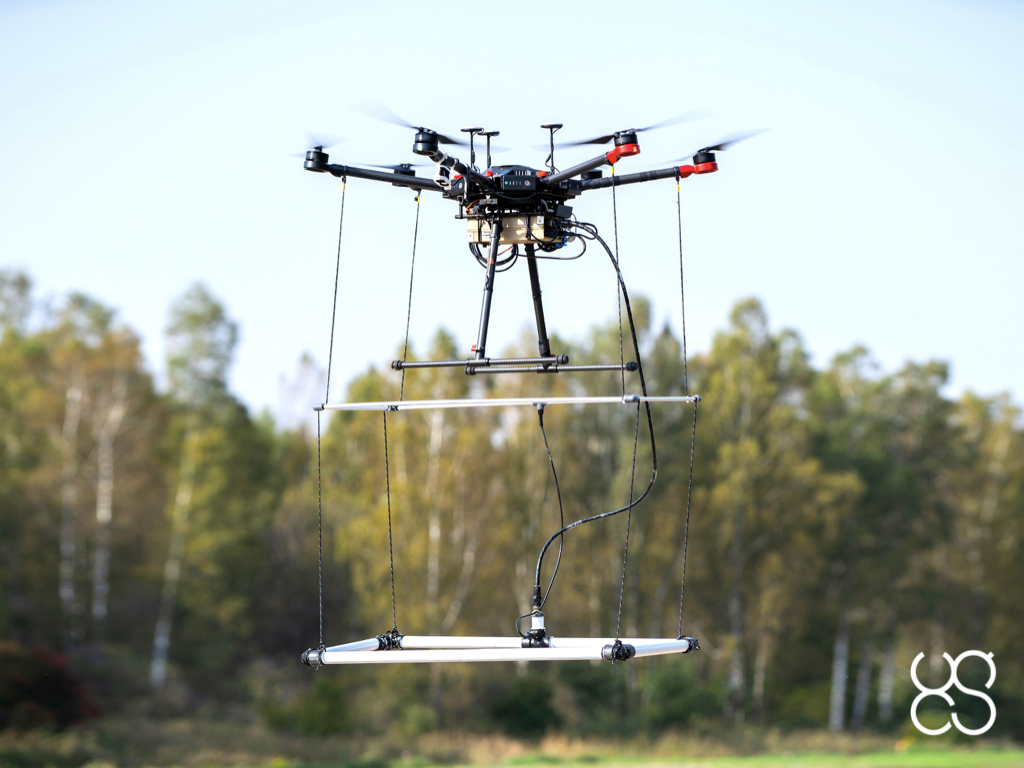
\includegraphics[width=\linewidth]{figs/Huirui/metal_detector_drone.png}
        \caption{UAV-mounted metal detector system\protect\footnotemark.}
        \label{fig:metal_detector_drone}
    \end{subfigure}
    \hfill
    \begin{subfigure}[b]{0.48\linewidth}
        \centering
        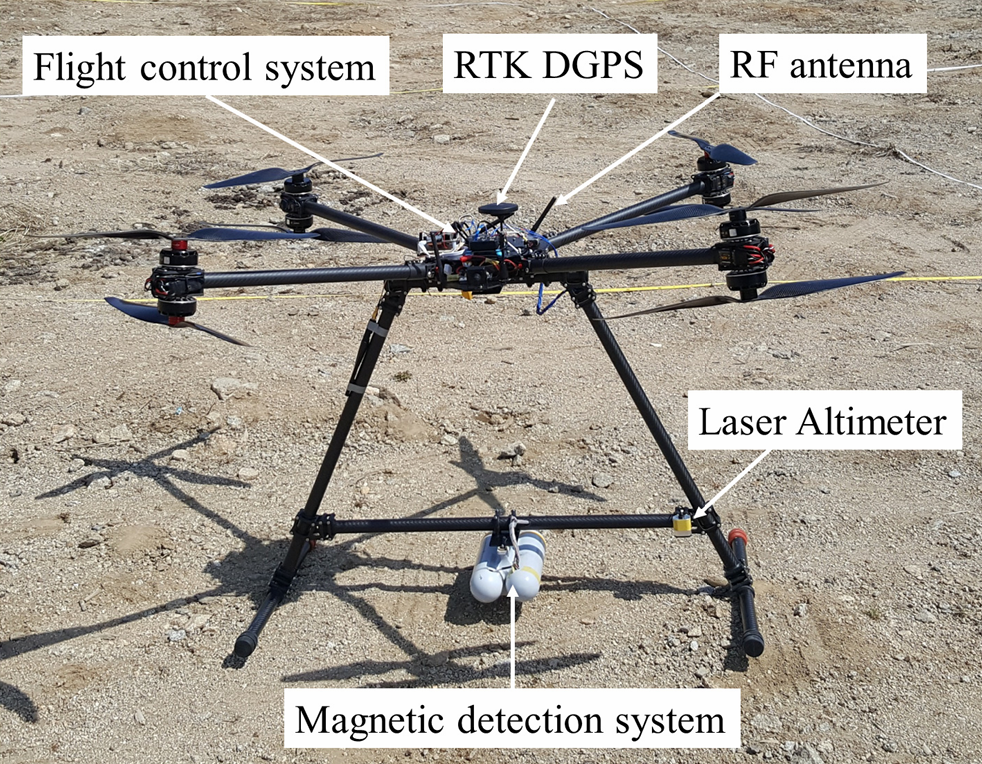
\includegraphics[width=\linewidth]{figs/Huirui/magnetometer_drone.png}
        \caption{Drone-based magnetometer platform~\cite{yoo2020drone}.}
        \label{fig:magnetometer_drone}
    \end{subfigure}
    \caption{Examples of UAV platforms integrating electromagnetic sensors for landmine detection.}
    \label{fig:emi_uav_examples}
\end{figure}

\footnotetext{\url{https://www.sphengineering.com/news/sph-engineering-introduces-the-drone-integrated-metal-detection-system}}

\paragraph{Radiowave and Microwave-Based Systems}

Ground Penetrating Radar (GPR) is a non-invasive geophysical technique that uses electromagnetic waves in the microwave frequency range (typically from several hundred MHz to a few GHz) to detect subsurface anomalies~\cite{gichd2006guidebook}. Unlike EMI-based systems, which respond to conductive or magnetic properties, GPR is sensitive to variations in the dielectric properties of materials~\cite{Gooneratne2004ARO}. It operates by transmitting short-duration radio pulses into the ground via a wideband antenna. When these pulses encounter boundaries between materials with different dielectric constants—such as between soil and a buried landmine—they are partially reflected. The reflected signals are then captured by a receiving antenna, and the time delay and intensity are analyzed to estimate the depth, shape, and dielectric contrast of subsurface targets~\cite{alqudsi2021review, paik2002image}.

As the antenna is moved across the ground, successive measurements are combined to construct two-dimensional slices (radargrams) or even three-dimensional volumetric representations of the subsurface~\cite{Bruschini1997ASO}. The effectiveness of GPR depends heavily on the contrast between the dielectric properties of the object and the surrounding soil. High-frequency systems offer better resolution and are more suited for detecting small anti-personnel mines, while lower-frequency systems provide deeper penetration but at the cost of detail~\cite{gichd2006guidebook}.

\textbf{Strengths:} One of GPR’s major strengths is its ability to detect both metallic and non-metallic mines, including those with plastic casings, by sensing changes in dielectric properties~\cite{Gooneratne2004ARO}. Unlike metal detectors, GPR systems are relatively insensitive to small surface metallic debris, which helps reduce false alarm rates~\cite{gichd2006guidebook}. They also provide useful information about object depth and shape, and can generate cross-sectional or 3D images of the subsurface~\cite{Bruschini1997ASO}. GPR is widely used in archaeological surveys, utility mapping, and geology, and is well understood in terms of commercial deployment and signal processing. Modern GPR systems are compact, lightweight, and pose no radiation hazard due to their low-power operation~\cite{gichd2006guidebook}.

\textbf{Limitations:} The main limitations of GPR lie in its sensitivity to soil conditions. High soil moisture, clay content, or rough surface topology can cause strong attenuation of the radar signal, making it difficult to detect shallow or low-contrast targets~\cite{Gooneratne2004ARO}. Performance can also degrade in dry, homogeneous soils due to insufficient dielectric contrast~\cite{robledo2009survey}. The detection of small anti-personnel mines can be particularly challenging if their signal is masked by surface reflections. Additionally, GPR systems require careful tuning of frequency to balance resolution and penetration depth, and are susceptible to signal distortion caused by subsurface clutter such as rocks, roots, or air pockets~\cite{cardonalandmine}.

\textbf{Drone-Based Applications:} GPR has been widely explored for drone integration due to its capability to detect plastic-cased mines and to provide volumetric subsurface data. UAV-mounted GPR systems typically use lightweight ultra-wideband (UWB) antennas and operate at low altitude to maintain signal fidelity. Applications include detecting anti-tank and anti-personnel mines in varied terrain types, including sand, loam, and clay\footnote{\url{https://www.sphengineering.com/integrated-systems/technologies/gpr}}~\cite{vsipovs2020lightweight,cerquera2017uav,fernandez2018synthetic,amiri2012feasibility,safarov2022detection,vsipovs2020lightweight,colorado2017integrated,schreiber2019advanced,pongrac2022advanced,garcia2020airborne,prager2019application,garcia2019autonomous,burr2018design,fernandez2021development,colorado2017low,lee2023modeling,sipos2017drone,garcia2022safedrone,almutiry2020uav,schartel2018uav,bahnemann2022under,garcia2022validation,chen2023ground}. Figure~\ref{fig:gpr_uav_examples} shows two UAV-based implementations of GPR for landmine detection.

\begin{figure}[h!]
    \centering
    \begin{subfigure}[b]{0.48\linewidth}
        \centering
        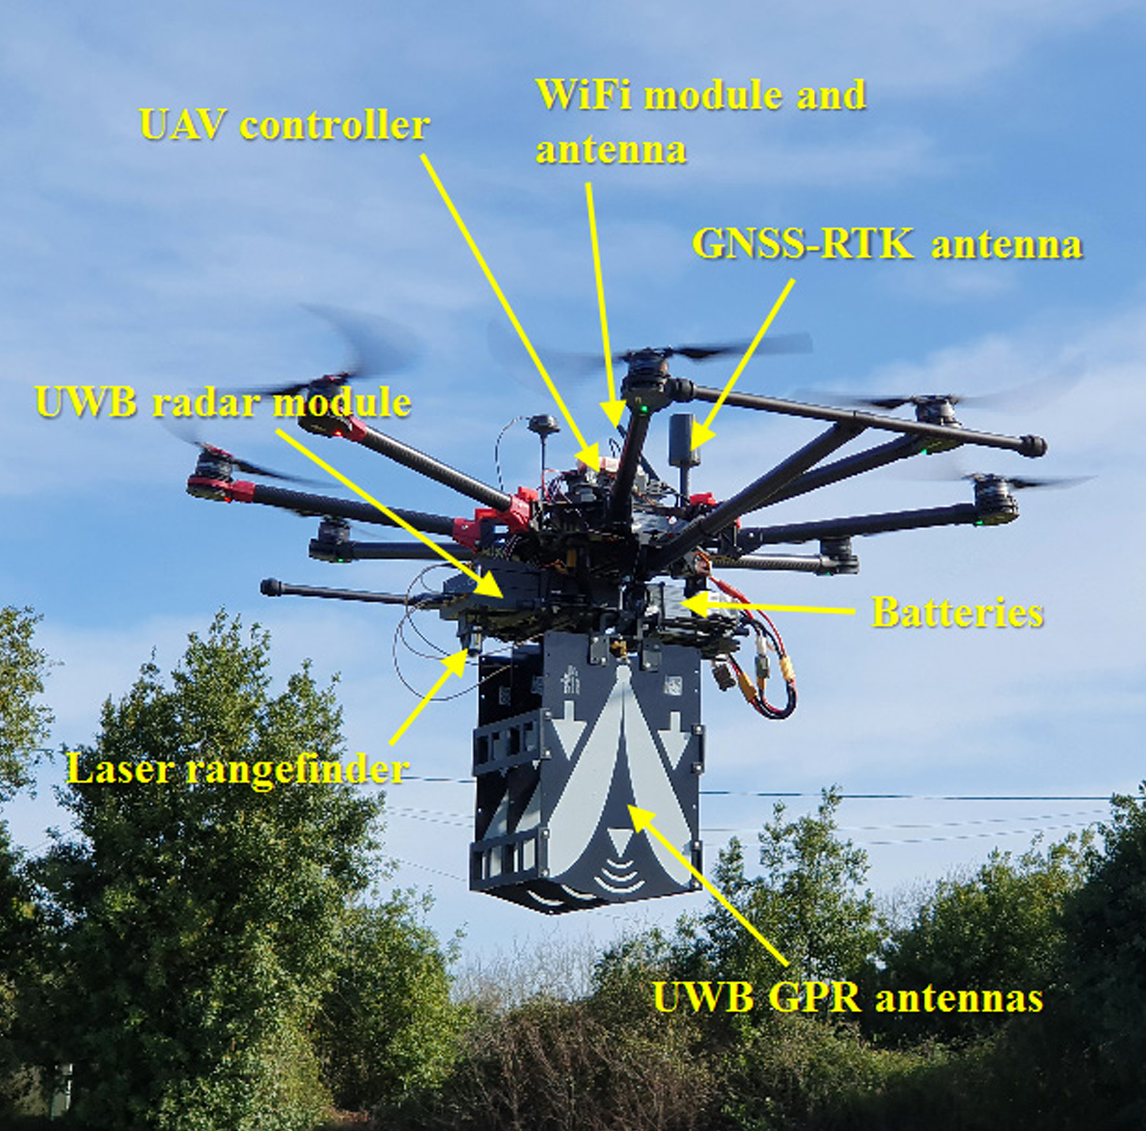
\includegraphics[width=\linewidth]{figs/Huirui/gpr_drone1.png}
        \label{fig:gpr_drone1}
    \end{subfigure}
    \hfill
    \begin{subfigure}[b]{0.48\linewidth}
        \centering
        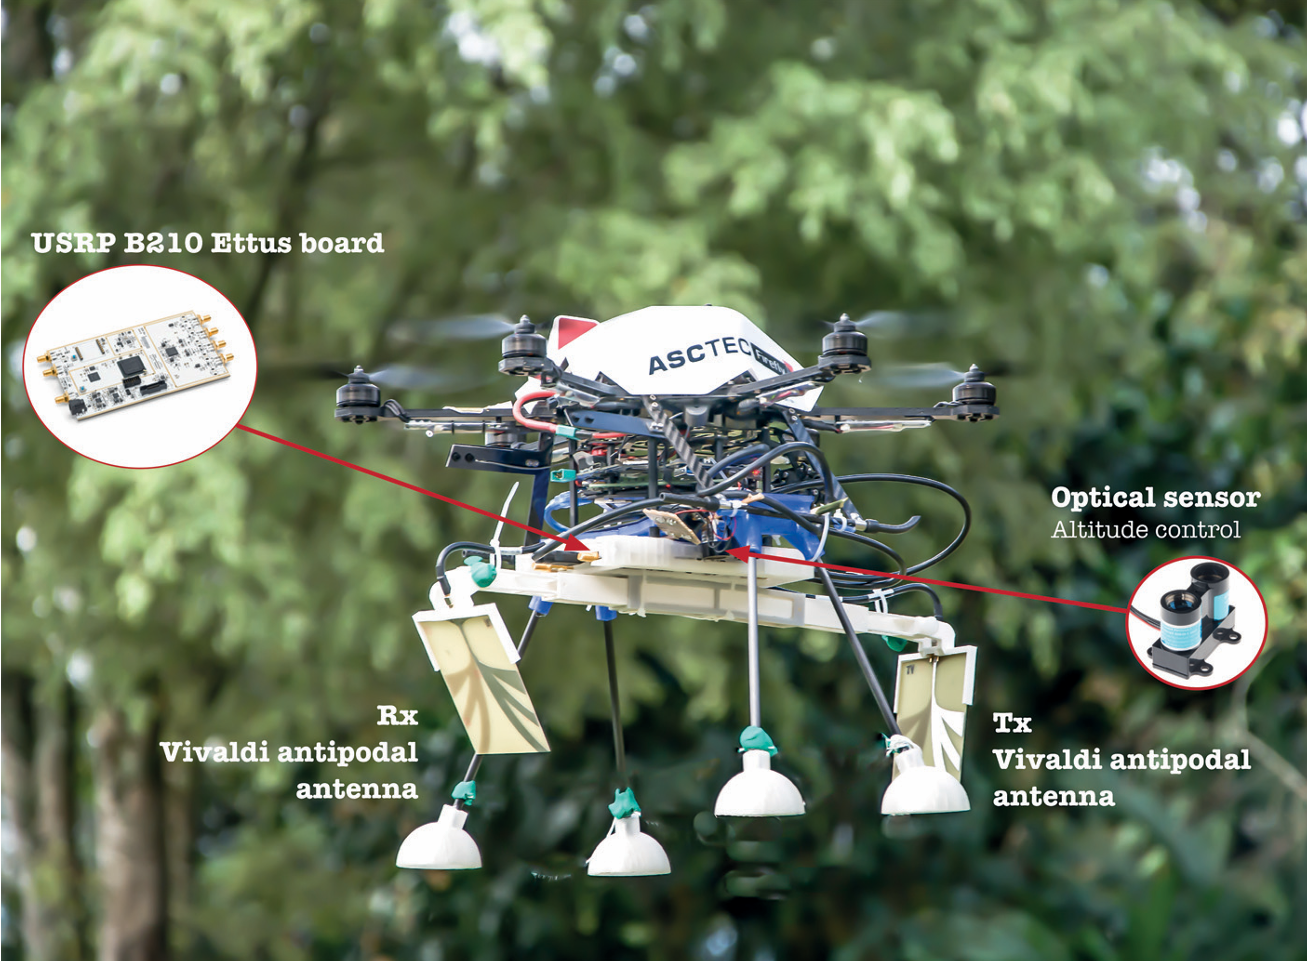
\includegraphics[width=\linewidth]{figs/Huirui/gpr_drone2.png}
        \label{fig:gpr_drone2}
    \end{subfigure}
    \caption{Examples of UAV platforms integrating GPR systems for landmine detection.~\cite{garcia2022safedrone,cerquera2017uav}}
    \label{fig:gpr_uav_examples}
\end{figure}

\subsection{Thermal Camera}

\subsubsection{Key Parameters}
- Wavelength range, frame rate, resolution, and altitude impact.

\subsubsection{Theoretical Considerations}
- Factors affecting thermal signature (e.g., burial depth, surface heating).

\subsubsection{Example Hardware and Final Selection}
- Summary of camera options and rationale for choice.

\subsubsection{Sensor Operation and Flight Parameter Configuration}
- Flying height, scanning resolution, and field of view.

- Guidelines from theory and past work to inform drone altitude and speed.
\subsection{Ground Penetrating Radar}\label{GPR_system}

\subsubsection{Fundamentals of GPR}\label{GPR_fundamental}

\gls{GPR} is a non-invasive subsurface sensing technique that detects buried objects by emitting \gls{EM} waves and analyzing their reflections. A typical \gls{GPR} system is consisted of a wideband antenna and an active sensor. The antenna emits \gls{EM} waves into the ground, and reflections are captured where there is a contrast in dielectric properties, like between soil and a buried landmine~\cite{paik2002image}.

The presence and depth of subsurface objects are inferred from discontinuities in the round-trip signal. The time delay $\Delta t$ between transmission and reception is used to estimate the distance $R$ to the reflecting object by \( R = \frac{v \cdot \Delta t}{2}\) where $v$ is the wave velocity in the medium depending on soil properties~\cite{paik2002image}.

To visualize \gls{GPR} data, three types of scans are commonly used: \textbf{A-scan}, \textbf{B-scan}, and \textbf{C-scan}. A-scans represent 1D reflections at a single point, showing signal amplitude versus time delay. B-scans combine a series of A-scans along a line to form a 2D cross-sectional view of the subsurface, while C-scans stitche together multiple adjacent B-scans to generate a volumetric 3D map of the ground. 

Figure~\ref{fig:gpr_coords} illustrates the 3D coordinate system used in \gls{GPR} scanning. A-scans are taken vertically into the ground at positions $(x’, y’)$. Moving the sensor along the $x$-axis forms a B-scan, and sweeping across $y$-axis yields a C-scan. A sample B-scan image is shown in Figure~\ref{fig:gpr_bscan}, where hyperbolic reflection patterns indicate buried objects~\cite{paik2002image}.

\begin{figure}[h!]
    \centering
    \begin{subfigure}[b]{0.48\linewidth}
        \centering
        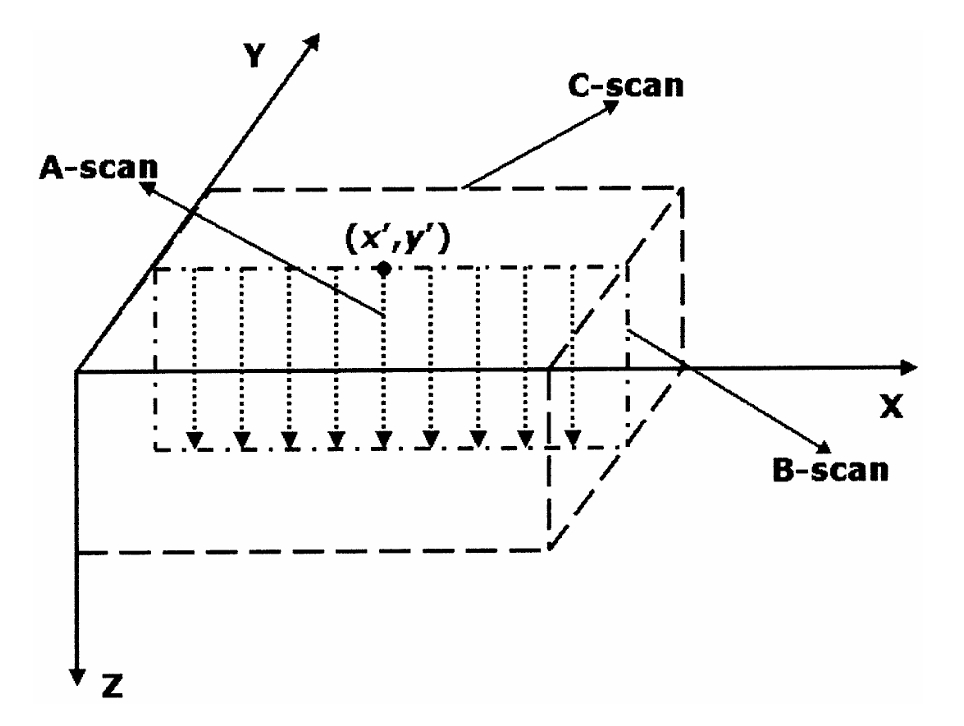
\includegraphics[height=5cm]{figs/Huirui/gpr_coords.png}
        \caption{Coordinate convention for GPR scanning.}
        \label{fig:gpr_coords}
    \end{subfigure}
    \hfill
    \begin{subfigure}[b]{0.48\linewidth}
        \centering
        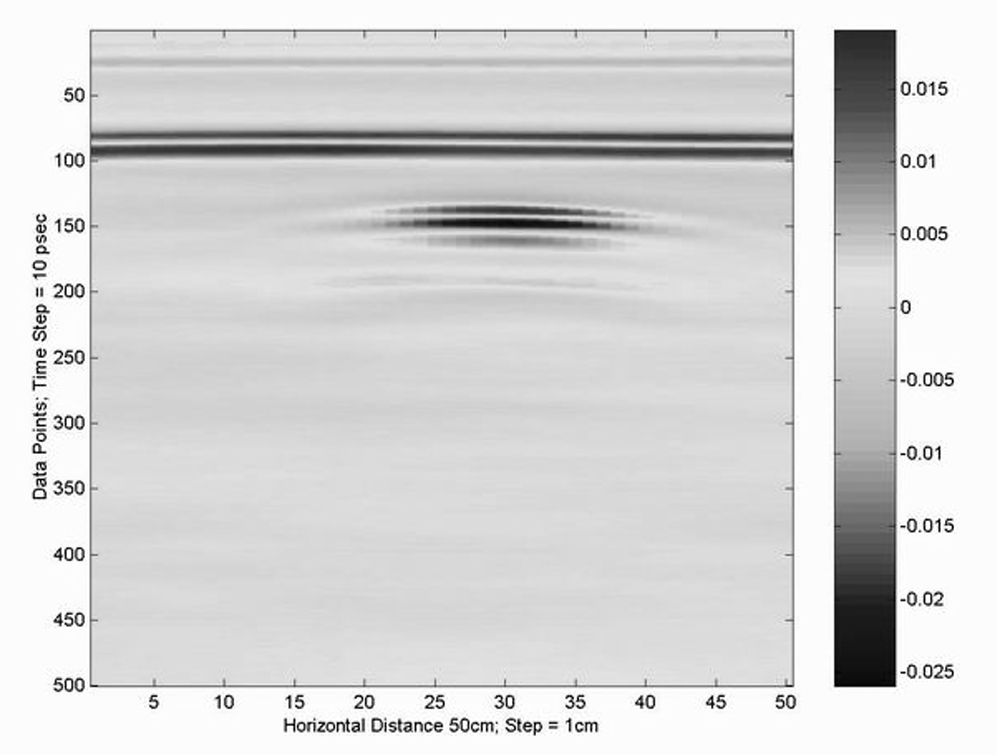
\includegraphics[height=5cm]{figs/Huirui/gpr_bscan.png}
        \caption{Example of a B-scan.}
        \label{fig:gpr_bscan}
    \end{subfigure}
    \caption[Visualization of GPR data acquisition and interpretation]{Visualization of GPR data acquisition and interpretation~\cite{paik2002image}.}
\end{figure}

Since our project focuses on localizing and estimating the depth of landmines rather than reconstructing their full 3D geometry, we collect and process only \textbf{B-scan} data from the \gls{UAV} \gls{GPR} platform.




\subsubsection{GPR Performance Factors}\label{GPR_Factors}

The performance of a \gls{GPR} system for \gls{UAV}-based landmine detection depends on a variety of factors that influence its resolution, penetration depth, and system complexity. These include waveform generation methods, operating frequency and bandwidth, spatial resolution metrics, antenna design, signal processing techniques such as \gls{SAR}, and orientation of the radar with respect to the ground surface. This section outlines the main design parameters and discusses their implications for airborne \gls{GPR} deployment.


\paragraph{Waveform Type}

The waveform type determines how \gls{GPR} transmits and receives \gls{EM} signals plays a critical role in determining resolution, hardware requirements, and system robustness. The three most common waveform types are summarized below:

\begin{itemize}
    \item \textbf{Impulse (pulsed)} \gls{GPR} transmits ultra-short pulses with broad spectral content, enabling ultra-wideband (UWB) operation and high-resolution imaging. These systems are elatively simple and cost-effective but require a \gls{ADC} or a subsampling receiver to process the wide bandwidth~\cite{chen2023ground,sipos2017drone}.

    \item \textbf{\gls{FMCW}} \gls{GPR} emits a continuous chirp signal with linearly increasing frequency over time. This approach offers better average transmitted power and improved \gls{SNR}, but requires more complex hardware and is more vulnerable to phase noise and motion errors~\cite{burr2018design}.
    
    \item \textbf{\gls{SFCW}} \gls{GPR} steps through discrete frequencies and collects reflections in the frequency domain. The data are then converted into time-domain signals via inverse Fourier transform. While achieving high \gls{SNR} and reduced \gls{ADC} requirements, \gls{SFCW} systems often perform poorly in \gls{UAV} applications due to weak ground coupling and strong surface reflections~\cite{tronca2018comparison}.
\end{itemize}


\paragraph{Centre Frequency, Bandwidth, Resolution, and Penetration Depth}

The centre frequency and bandwidth of a radar signal are key parameters about the \gls{GPR} system’s resolution and penetration depth. 

In general, lower frequencies (e.g., < 1 GHz) enhance penetration depth but limit resolution. Higher frequencies (e.g., > 2--3 GHz) improve resolution but attenuate quickly, especially in moist or conductive soils. For example, a \gls{GPR} operating at 3~GHz may penetrate up to 0.5 m in dry soil, but only a few centimeters in wet environments~\cite{9758040}. This trade-off is illustrated in Figure~\ref{fig:freq_tradeoff}, where increasing frequency improves resolution (represented as gray circles becoming smaller) at the cost of reduced sensing depth.

\begin{figure}[H]
    \centering
    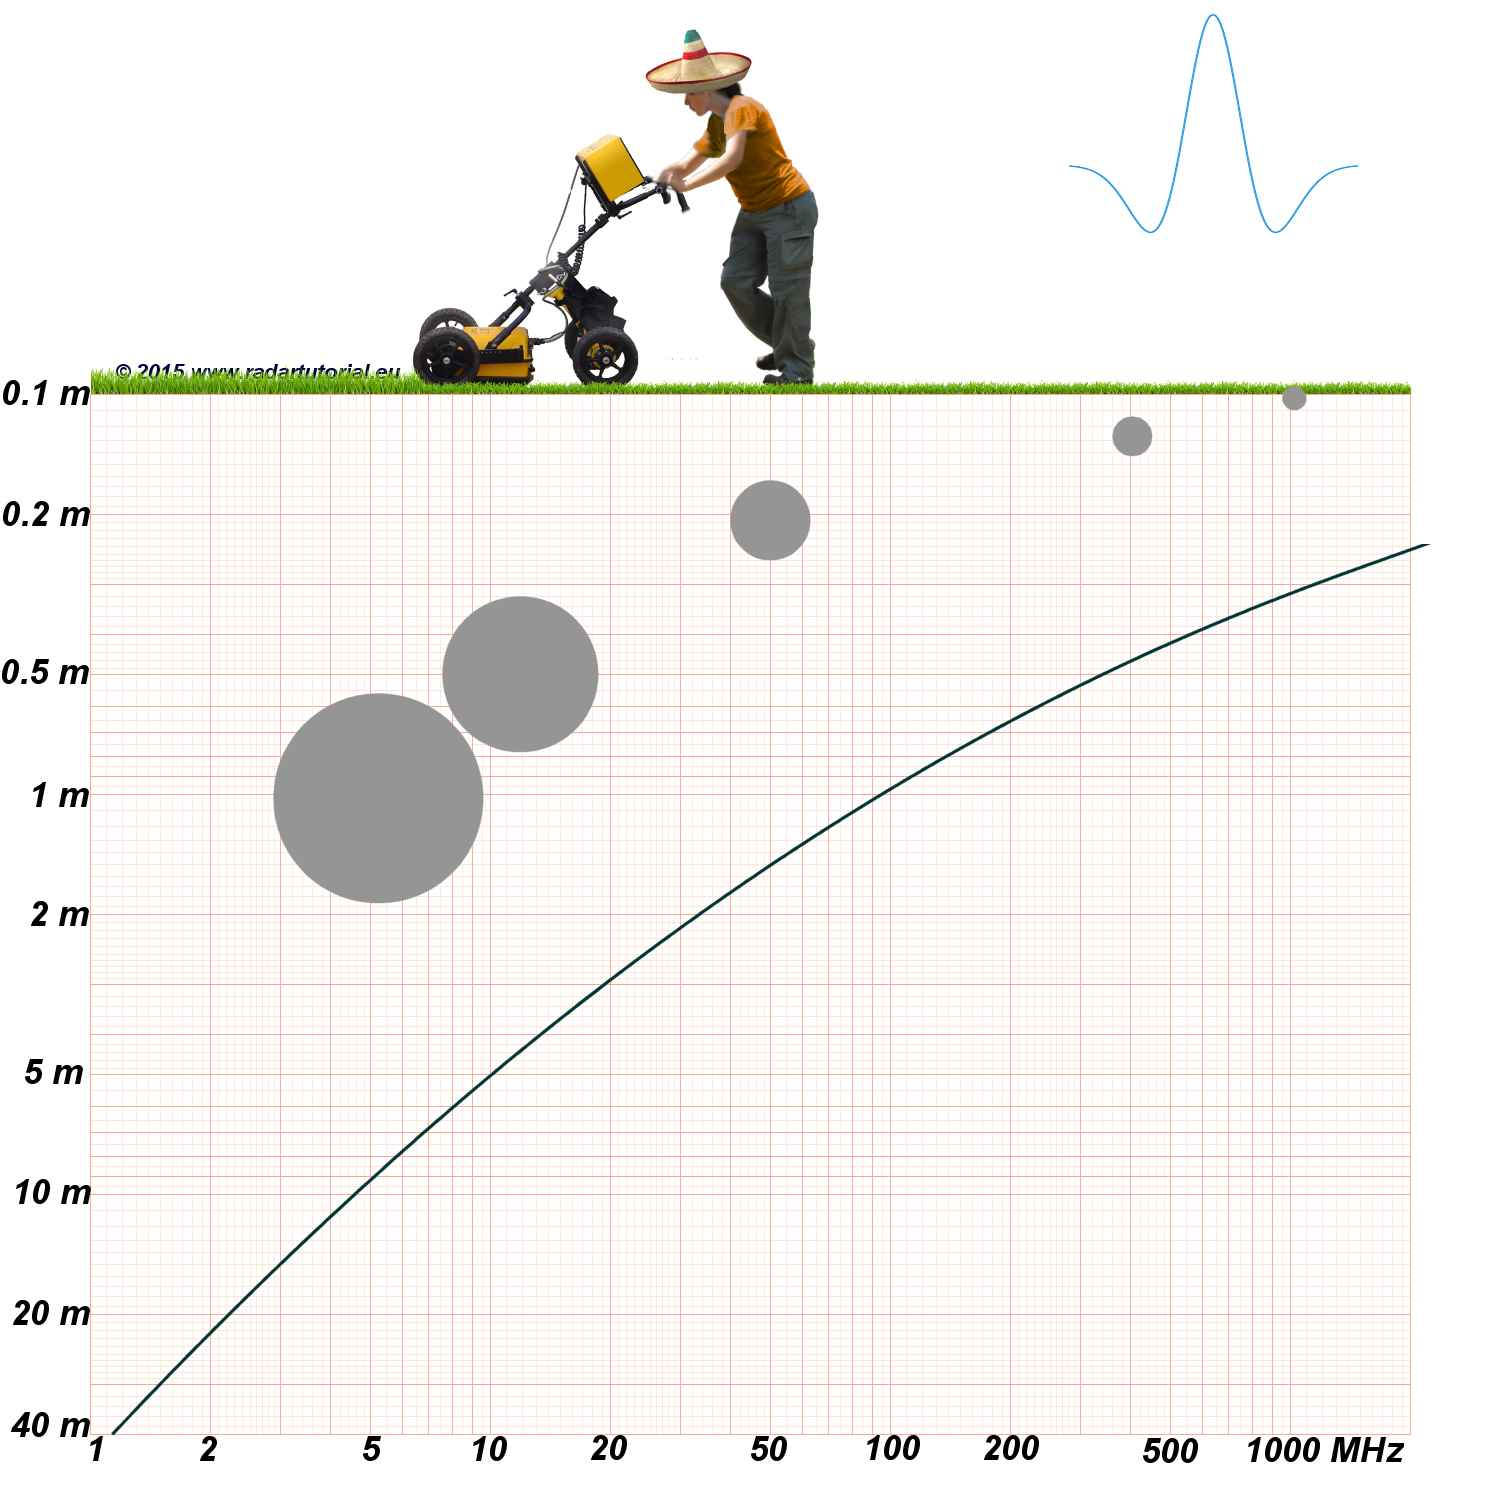
\includegraphics[width=7cm]{figs/Huirui/freq_tradeoff.png}
    \caption[Frequency, resolution, and penetration depth trade-off]{Frequency, resolution, and penetration depth trade-off\protect\footnotemark.}
    \label{fig:freq_tradeoff}
\end{figure}
\footnotetext{\url{www.radartutorial.eu}}


The radar’s bandwidth, defined as the difference between the maximum and minimum frequencies $B = f_{\text{max}} - f_{\text{min}}$, determines the system’s range (or depth) resolution $\Delta r$, which is the ability to distinguish between objects at different depths along the same vertical axis. In free-space conditions where the wave velocity $v_p = c$ (the speed of light), the range resolution $\Delta r$ is approximated by: \(\Delta r = \frac{c}{2B}~\cite{9758040}\)

Cross-range or lateral resolution $\Delta l$ defines the radar’s ability to distinguish adjacent objects at the same depth. It depends on the central wavelength $\lambda_c$, aperture size $L_{\text{ap}}$, and antenna-to-target distance $R$, and is approximated as: \(\Delta l = \frac{R \cdot \lambda_c}{L_{\text{ap}}}~\cite{9758040}\)



\paragraph{Antenna Size}

The physical size of a \gls{GPR} antenna is closely linked to the operating frequency, with lower frequencies requiring larger antennas. A rough estimate of the minimum antenna length is given by: \(L_{\text{antenna}} \approx \frac{\lambda_{\text{min}}}{2}\), where $\lambda_{\text{min}}$ is the wavelength of the minimum \gls{GPR} frequency~\cite{burr2018design}.

This relationship introduces a trade-off between penetration depth and physical size: lower frequencies penetrate deeper but require larger antennas, which may exceed the payload and form-factor limits of \gls{UAV} platforms.


\paragraph{SAR Processing}

Traditional \gls{GPR} systems have limited cross-range resolution due to the small sizes of antennas. \gls{SAR} addresses this limitation by coherently integrating radar echoes collected along the \gls{UAV}’s flight path, synthesizing a larger aperture, and significantly improving lateral resolution. This is especially beneficial for \gls{UAV}-based \gls{GPR} where antenna size and weight are constrained~\cite{9758040}.

Among \gls{SAR} algorithms, \textbf{\gls{BP}} is particularly suited for \gls{UAV} applications due to its robustness to irregular trajectories and non-uniform sampling. \gls{BP} operates by summing radar echoes along computed time-delay curves for each focal point. As shown in Figure~\ref{fig:bp_geometry}, radar signals $e_1(x_p, t)$ are collected at multiple \gls{UAV} positions $x_p$. The round-trip travel time $\tau_{m,n,p}$ from the transmitter to a target point $(x_n, z_m)$ and back is used to time-shift and coherently sum these signals by \(e_2(x_n, z_m) = \sum_{p=1}^{P} e_1(x_p, \tau_{m,n,p})\) and \(\tau_{m,n,p} = \frac{2R_a}{c} + \frac{2R_b}{v}\) where $R_a$ and $R_b$ are distances through air and soil respectively, $c$ is the speed of light, and $v$ is the wave velocity in soil. This delay-and-sum approach transforms hyperbolic reflections in conventional B-scans (like Figure~\ref{fig:gpr_bscan}) into focused point targets, improving subsurface interpretability. However, the method is computationally intensive and not ideal for real-time onboard processing~\cite{lei2014multi}.

\begin{figure}[H]
    \centering
    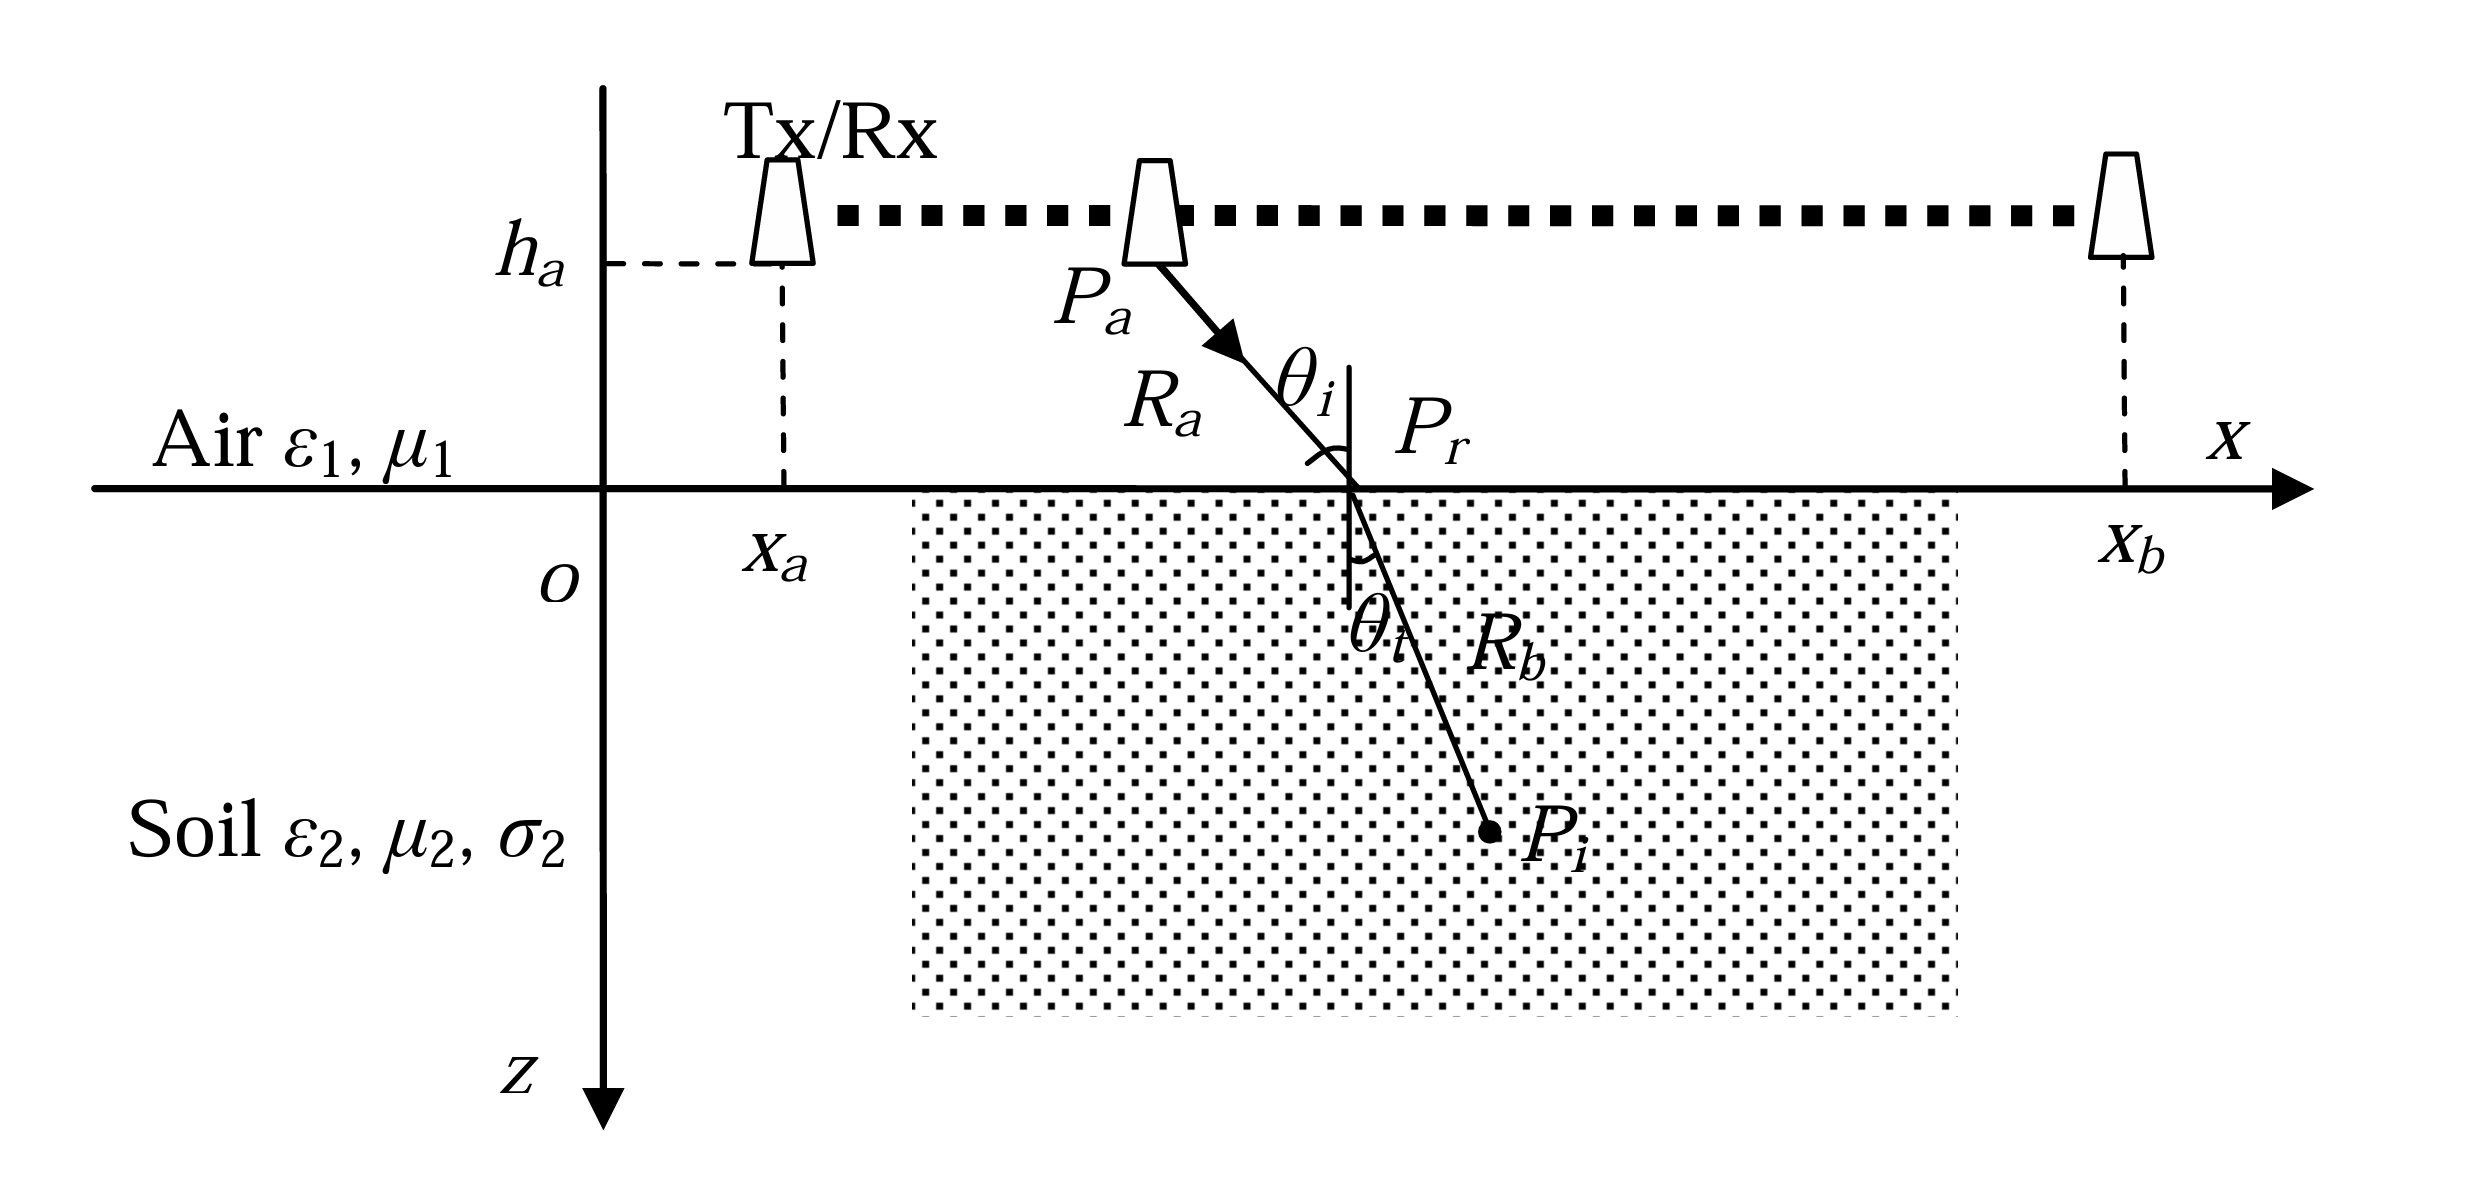
\includegraphics[height=5cm]{figs/Huirui/bp_geometry.png}
    \caption[BP SAR imaging geometry]{Illustration of BP SAR imaging geometry~\cite{lei2014multi}.}
    \label{fig:bp_geometry}
\end{figure}


\gls{SAR} can operate in different beam-steering modes depending on coverage and resolution needs (Figure~\ref{fig:sar_modes}):

\begin{itemize}
    \item \textbf{Stripmap \gls{SAR}} maintains a fixed beam relative to the \gls{UAV}, illuminating a continuous swath as the platform moves forward, which offers a balance between area coverage and resolution~\cite{moreira2013tutorial}.
    \item \textbf{Scan \gls{SAR}} periodically steers the beam to cover multiple adjacent swaths, increasing area coverage at the cost of reduced resolution~\cite{moreira2013tutorial}.
    \item \textbf{Spotlight \gls{SAR}} keeps the beam focused on a single target area, maximizing resolution but limiting area coverage~\cite{moreira2013tutorial}.
\end{itemize}

\begin{figure}[H]
    \centering
    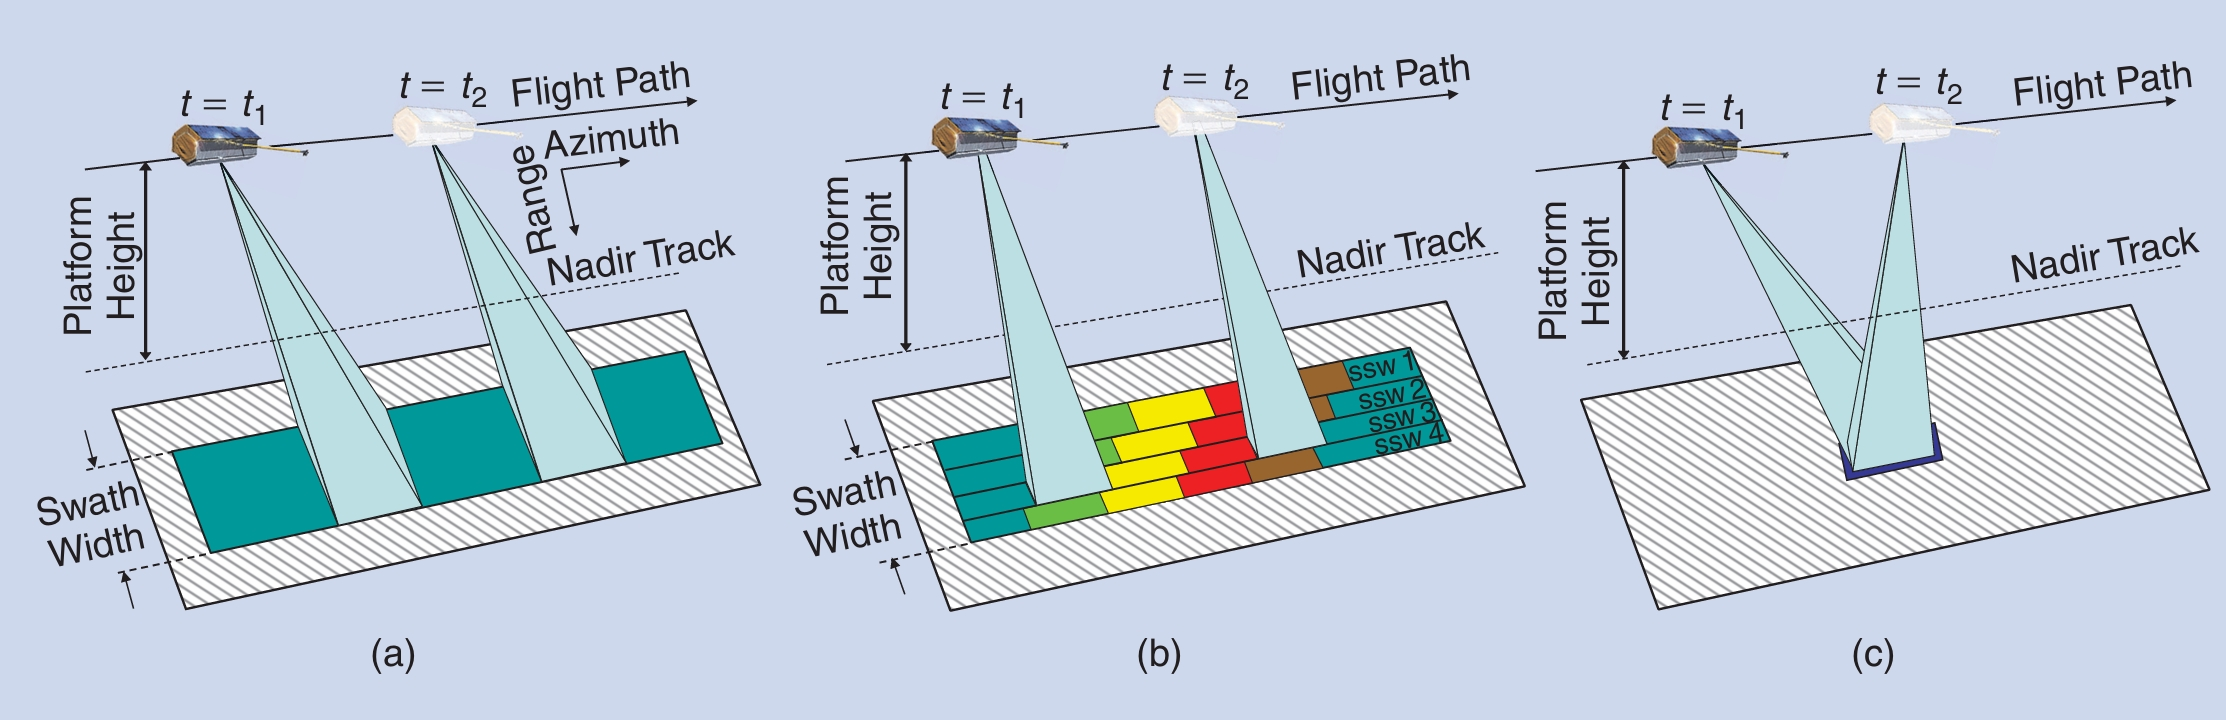
\includegraphics[height=4cm]{figs/Huirui/sar_modes.png}
    \caption[SAR operation modes]{Different SAR operation modes: (a) Stripmap SAR, (b) Scan SAR, and (c) Spotlight SAR~\cite{moreira2013tutorial}.}
    \label{fig:sar_modes}
\end{figure}


\paragraph{Radar Orientation}

The orientation of the \gls{GPR} antenna on a \gls{UAV} plays a critical role in determining both imaging performance and ease of integration. Two common configurations are illustrated in Figure~\ref{fig:GPR_Ori_modes}:

\begin{itemize}
    \item \textbf{\gls{FLGPR}} or \textbf{Side-Looking \gls{GPR}} emits waves obliquely into the ground, which reduces surface clutter. However, it receives weak backscattered signals from buried objects, requiring high dynamic range receivers and precise beam alignment~\cite{garcia2020airborne}.

    \item \textbf{\gls{DLGPR}} points antennas perpendicularly toward the ground, maximizing reflected signal strength from targets but becoming more sensitive to surface clutter~\cite{garcia2020airborne}.
\end{itemize}

\begin{figure}[H]
    \centering
    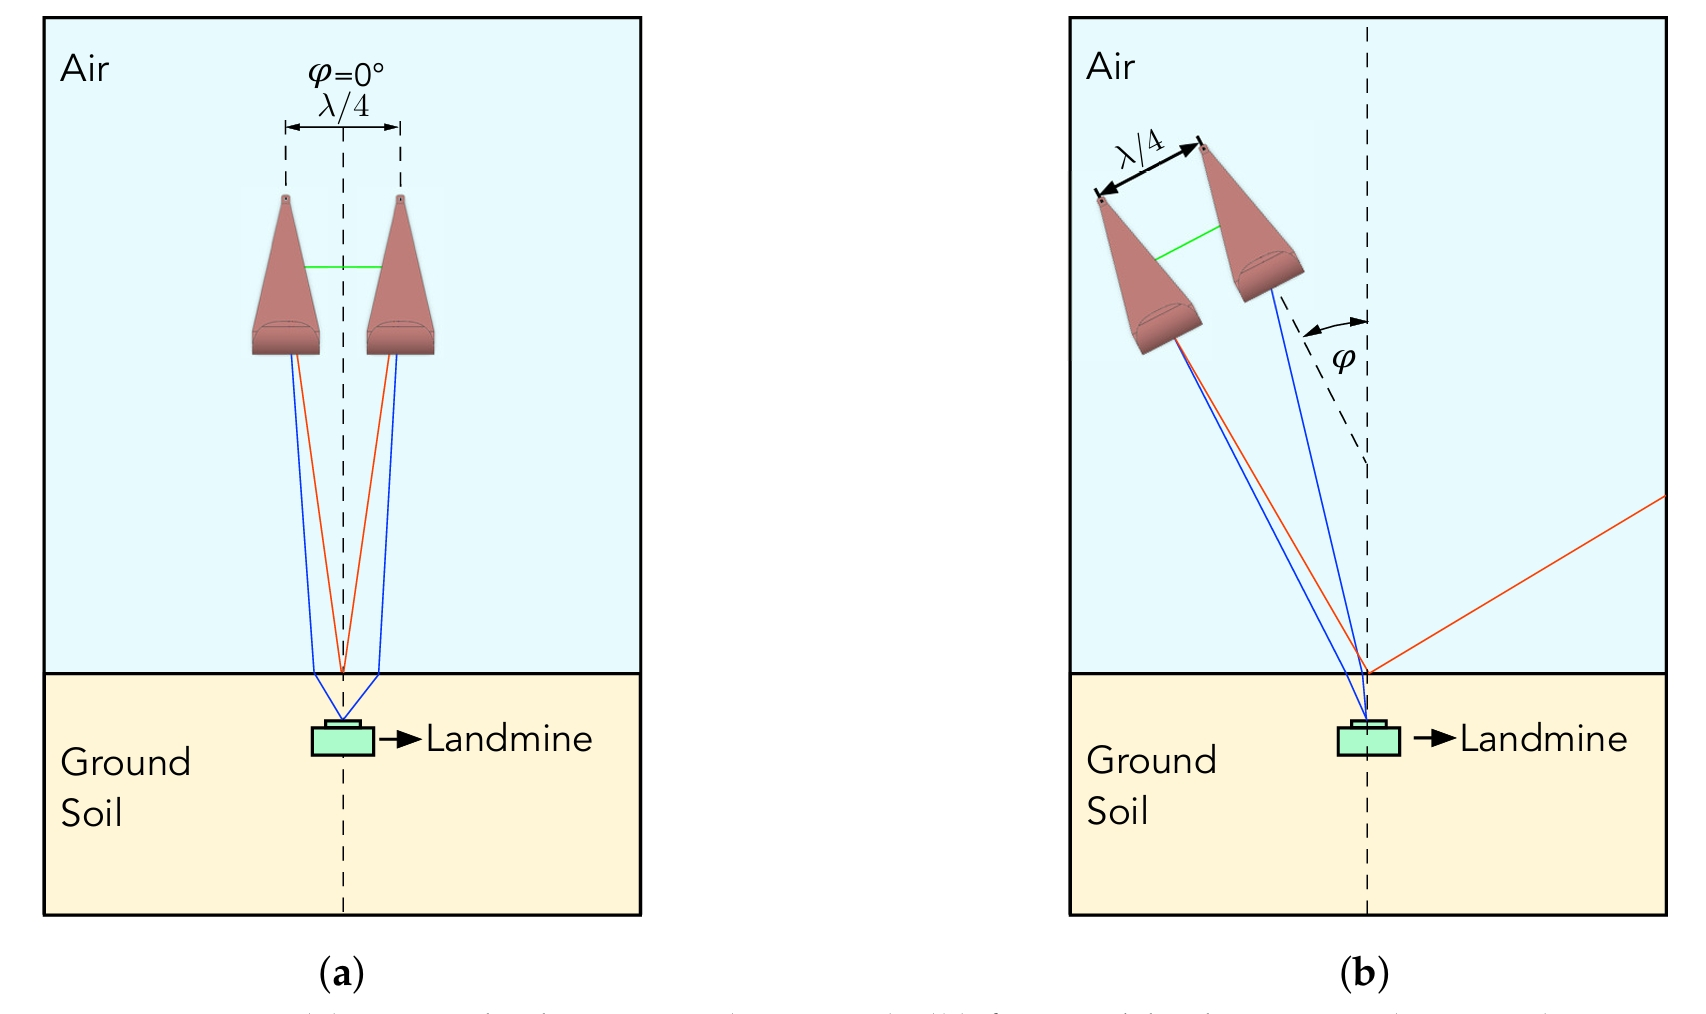
\includegraphics[height=6cm]{figs/Huirui/gpr_ori_modes.png}
    \caption[GPR orientations]{GPR orientations: (a) DLGPR, and (b) FLGPR~\cite{vsipovs2020lightweight}.}
    \label{fig:GPR_Ori_modes}
\end{figure}



\subsubsection{GPR System Design}\label{GPR_design}

While numerous \gls{GPR} architectures have been explored in previous research, most high-performance \gls{UAV}-based landmine detection systems rely on custom radar platforms. These typically incorporate \gls{SDR}, customized waveform generators, and advanced antenna arrays to maximize their environmental adaptability, resolution, and penetration~\cite{cerquera2017uav}.

In contrast, the focus of our project is to demonstrate the feasibility of integrating \gls{GPR} within a layered, multi-\gls{UAV} landmine detection framework. Given the constraints of time, budget, and hardware development, we propose the use of a \gls{COTS} impulse \gls{GPR} system for our initial implementation.

We select the \textbf{SPH Engineering Zond Aero 1000 MHz \gls{GPR}} (~1.8~kg\footnote{\label{Zond}\url{https://cdn.shopify.com/s/files/1/0596/9451/4353/files/RadSys_Zond_Aero_1000_NG_datasheet.pdf?v=1732295405}}). It operates in the 600–1300~MHz band with a center frequency of 1~GHz\textsuperscript{\ref{Zond}}, offering reasonable balance between resolution and penetration. Unlike high-frequency systems that offer fine detail at shallow depths, this system prioritizes deeper penetration—essential for detecting mines in compact or moist soils. Although its vertical resolution (around 10--15~cm) may not allow precise depth estimation, this is acceptable for our use case, where the primary goal is to confirm the existence rather than reconstruct detailed object geometry of the buried landmines.

The system uses a \textbf{\gls{DLGPR}} configuration, maximizing reflected signal power from targets and simplifying hardware integration. While \gls{DLGPR} does introduce surface clutter due to strong air–ground reflections, it can be mitigated through signal processing techniques such as Singular Value Decomposition (SVD) and migration algorithms ~\cite{garcia2024comparison}. Furthermore, \gls{DLGPR} is the most widely adopted orientation in past \gls{UAV}-\gls{GPR} applications, supporting its practical reliability ~\cite{9758040}.

To improve lateral resolution and compensate for the limited range resolution of our low-frequency radar, we apply \gls{SAR} processing in \textbf{Stripmap} mode using a \textbf{\gls{BP}} algorithm. This enables continuous scanning without beam steering, reducing \gls{UAV} control complexity. Since coherent SAR imaging requires centimeter-level positioning accuracy to align radar returns across the UAV trajectory~\cite{fernandez2018synthetic}, we ensure this through the integration of a high-precision GNSS and IMU system, as described in section~\ref{sub_sub_section:tgt_component_selection}. Real-time processing is avoided due to the computational cost of \gls{BP}; instead, raw B-scans are geo-referenced and processed offline after each flight.

This system architecture based on a down-looking \gls{COTS} impulse radar at low-frequency operation with offline \gls{SAR} processing provides a realistic and effective foundation for our system’s initial deployment. It balances feasibility with performance, while leaving room for future upgrades such as real-time \gls{SDR} control or custom radar development in subsequent project phases.



\subsubsection{GPR System Flight Configuration}\label{GPR_flight}

In our system, the \gls{GPR} drone is designed to fly at an altitude around \textbf{2~m}. This low flight height ensures a balance between maximizing power coupling into the ground and maintaining safe clearance for autonomous operations, consistent with previous \gls{DLGPR} studies on \gls{UAV} landmine detection ~\cite{schartel2018uav,9758040}.

As illustrated in Figure~\ref{fig:swath_geometry}, for our \gls{DLGPR} system ($\alpha = 90^\circ$), assuming a beamwidth (the angle between near range and far range) of $\theta = 45^\circ$, the effective swath width $W$ can be derived geometrically as \(W = 2H \cdot \tan\left(\frac{\theta}{2}\right)\). For $H = 2$~m,  $W = 1.65$~m. This value defines the effective width of ground coverage per flight strip.

\begin{figure}[H]
    \centering
    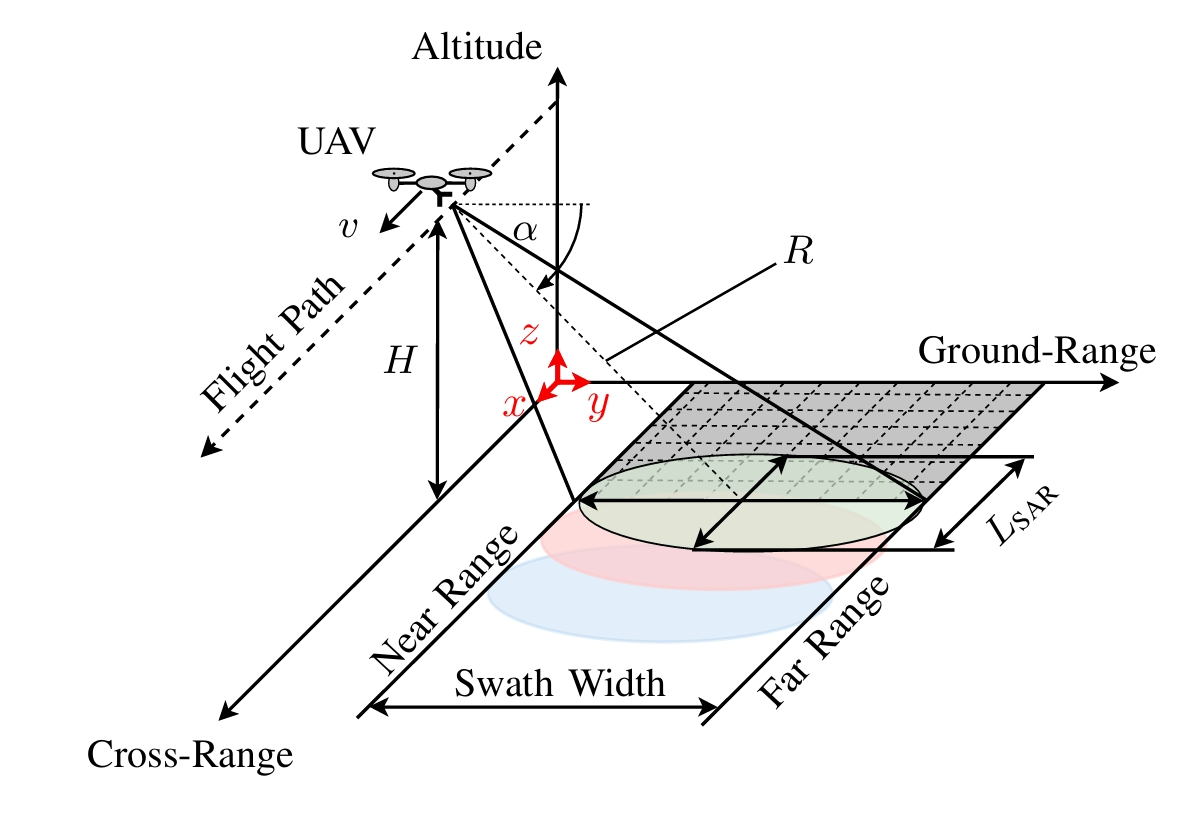
\includegraphics[height=6cm]{figs/Huirui/gpr_swath}
    \caption[Stripmap SAR geometry]{Illustration of the stripmap SAR geometry.~\cite{schartel2018uav}.}
    \label{fig:swath_geometry}
\end{figure}

To enable effective \gls{SAR} reconstruction using the \gls{BP} algorithm, radar acquisition points must satisfy the Nyquist sampling rate, which requires that the maximum spacing $\Delta x$ between successive measurements does not exceed half the wavelength corresponding to the system's maximum radar frequency: \(\Delta x \leq \frac{\lambda_{\text{min}}}{2}\)~\cite{9758040}.

For our system with a maximum operating frequency of 1.3~GHz, the minimum wavelength is approximately 23~cm, resulting in a maximum sampling interval of \textbf{11.5~cm}. Given the estimated thermal camera coverage of 9 m × 7 m mentioned in section before, assuming a zig-zag path with overlapping swath like Figure~\ref{fig:swath_geometry}, a total of \textbf{332 points} are required to fully sample one thermally flagged region. 
\subsection{Sensor Integration}

\subsubsection{Sensor Integration and Data Handling}
- Data interfaces and storage solutions (e.g., onboard SD logging).

- Software hooks for starting/stopping recording and syncing data with GPS.

\subsubsection{Preprocessing and Onboard Processing}
- Initial data cleaning or transformation (e.g., filtering GPR signals).

- Localization tagging for thermal and radar data.

- Mention potential for real-time or offline processing.

\newpage
\pagenumbering{arabic}
\fancyhead[C]{Rory Millard}
\section{Computer Vision} \label{computervision}

\subsection{Thermal Computer Vision}

This is the thermal computer vision subsection
\subsection{Thermal Simulations}

This is the thermal simulations subsection

\subsubsection{Governing Equations}
Unsteady Heat Equation

The general form of the 3D unsteady heat equation in Cartesian coordinates is:

\begin{equation}
    c_p \rho \frac{\partial T}{\partial t} = 
    \frac{\partial}{\partial x} \left( k \frac{\partial T}{\partial x} \right) + 
    \frac{\partial}{\partial y} \left( k \frac{\partial T}{\partial y} \right) + 
    \frac{\partial}{\partial z} \left( k \frac{\partial T}{\partial z} \right)
\end{equation}


where:
\begin{itemize}
    \item \( T(x,y,z,t) \) is the temperature field,
    \item \( k(x,y,z,t) \) is the thermal conductivity,
    \item \( \rho(x,y,z,t) \) is the mass density,
    \item \( c_p (x,y,z,t) \) is the specific heat capacity.
    
\end{itemize}

For piecewise constant properties $\rho, k, c_p$ this can be written as

\begin{equation}
    \frac{\partial T}{\partial t} = \alpha \left( \frac{\partial^2 T}{\partial x^2} + \frac{\partial^2 T}{\partial y^2} + \frac{\partial^2 T}{\partial z^2} \right)
\end{equation}

which can be compactly written as

\begin{equation}
    \frac{\partial T}{\partial t} = \alpha \nabla^2 T
\end{equation}



Where \( \alpha(x,y,z,t) := \frac{k}{\rho c_p}\) is the thermal diffusivity.


\subsection{Radar Computer Vision}

This is the radar computer vision subsection
\subsection{Radar Simulations}

This is the radar simulations subsection

\subsection{Data Fusion}

This is the data fusion subsection

\newpage
\fancyhead[C]{Rory Millard}
\section{Sensor Fusion} \label{fusion}



\subsection{Overview of Fusion} \label{fusion_overview}

    \noindent The late stage fusion approach was introduced in Section \ref{compvis_intro}. It is justified on the grounds of simplicity; by processing each sensor's data through individual YOLO models before merging, the network architectures are simpler. The networks can be retrained in parallel, and single points of failure are removed. 
    


    \noindent In this section, the outputs from the individual YOLO models are interpreted as probability maps, where the confidence value assigned by the YOLO model is equal to the probability of finding a landmine at that location, according to each sensor. The fusion algorithm combines the two probability maps, defined over the same geographical space, into a third map. This is done using the sensor data and environmental contextual data.

    Fusing the sensor outputs before the CNN is problematic due to irregular input sizes and the need for computationally intensive mosaicking algorithms that may introduce errors. Instead, the accurate position, pose and field of view metadata  is leveraged to project each YOLO output onto a common geographical grid. Given that these probability maps are inherently sparse (most of the probability map is zero, with occasional spikes over landmines), the projections are computationally efficient. Because the metadata is accurate, the overlapping regions of the projections will be small, and when they occur, a simple strategy—such as weighted averaging—suffices to resolve them.

    \subsubsection{The Precision-Recall Trade-off } \label{lossmatrix}

        Recall should be prioritized over precision, as a false negative in landmine detection is more dangerous than a false positive. However, no system can ensure 100\% recall, and so a mined region can never be 100\% safe. Therefore, reducing recall slightly in exchange  for a significant gain in precision can be advantageous, because the reduced recall has negligible operational impact, whilst the increased precision is associated with significant cost reduction.
\subsection{Fusion System Performance Bounds}\label{fusion_bounds}

    Independent of the specific fusion algorithm employed, the overall system performance is ultimately constrained by the intrinsic capabilities of the individual sensors. A Naive Bayes framework is adopted to establish performance estimates. The Naive Bayes approach assumes conditional independence between sensors, allowing for straightforward analytical expressions of posterior probabilities. While this simplification may not perfectly capture all sensor interactions, it provides tractable mathematics that yield conservative performance estimates; algorithms that are not limited by conditional independence, and have access to domain knowledge, will perform better than Naive Bayes for fusion.

    \subsubsection{Theoretical Framework}
        
        The following key parameters and their probabilistic interpretation, are defined: the prior mine density $\rho_0 = P(\text{Mine})$, the set of locations that have been flagged by the thermal sensor \(\mathcal{T}^+\), the thermal sensor's recall $R_T = P(\mathcal{T}^+\mid\text{Mine})$ , and its false positive rate $F_T = P(\mathcal{T}^+ \mid \overline{\text{Mine}})$. Similarly, the radar sensor is characterized by its recall $R_R$ and false positive rate $F_R$ with analagous interpretations. Following thermal scanning, the mine density in the flagged region ($\rho_1$), can be found with Bayes rule:
        \begin{equation}
        \rho_1 = P(\text{Mine} \mid \mathcal{T}^+) =\frac{P(\mathcal{T}^+\mid\text{Mine})P(\text{Mine})}{P(\mathcal{T}^+\mid\text{Mine})P(\text{Mine})+ P(\mathcal{T}^+\mid \overline{\text{Mine}})P(\overline{\text{Mine}})} =\frac{R_T \rho_0}{R_T \rho_0 + F_T (1 - \rho_0)}
        \end{equation}
        
        \paragraph{Mine Densities} 
        

            Note the use of mine densities (\(\rho\)) rather than the nominal precision values reported in Section \ref{compvis_implementation}. This is because of the class imbalance discussed in Section \ref{class_imbalance}. The nominal precision derived from an imbalanced dataset is misleading when applied to real-world conditions. Instead, a full Bayesian treatment that incorporates the prior distribution over mine density is used. This enables the accurate updating of mine density after thermal screening, giving \(\rho_1\), and then after radar verification, giving \(\rho_2\), thereby mitigating the effects of class imbalance.

    \subsubsection{Bounds on Precision and Recall}
    
        \paragraph{Precision} Under the Naive Bayes framework, the expected system precision after fusion equals the posterior mine density after both sensors have flagged an area. The radar sensor refines the density from $\rho_1$ to $\rho_2$, and the expected precision after fusion is:
        \begin{equation}
        \label{eq:rho_2}
        P_\text{F} = \rho_\text{2} = \frac{R_\text{R} \rho_\text{1}}{R_\text{R} \rho_\text{1} + F_\text{R} (1-\rho_\text{1})} \text{, where }         \rho_\text{1} = \frac{R_\text{T} \rho_\text{0}}{R_\text{T} \rho_\text{0} + F_\text{T} (1-\rho_\text{0})}.
        \end{equation}
        
         The upper bound is the radar's intrinsic precision $P_\text{R}$, giving \textbf{precision bounds of } $\rho_\text{2} \leq P_\text{sys} < P_\text{R}$
         
        \paragraph{Recall} The Naive Bayes system recall can similarly be found by considering the intrinsic recalls of each sensor, and is a lower bound on the true system recall. Because the radar sensor only scans regions flagged by the thermal sensor, the NB system recall is the product of the individual recalls \(R_\text{sys} = R_\text{T} R_\text{R}\), 
        which  cannot exceed $R_\text{T}$. This gives the \textbf{bounds on the fused system's recall as} $R_\text{T}R_\text{R}\leq R_\text{sys}< R_\text{T}$.
    
    \subsubsection{Naive Bayes Fusion: Quantifying Bounds} \label{Rory_quantifying_bounds}
    
        Using the YOLO model performance metrics in Table \ref{tab:sensor_comparison}, and a prior landmine density of 2\% ($\rho_0 = 0.02$), the following values are obtained: $R_T = 0.919,~ F_T = 0.15,~ R_R = 0.833,~ F_R = 0.085.$ These values are used to calculate the posterior density after thermal screening and subsequent radar scanning, using Equation \ref{eq:rho_2}:
        \[
        P_{sys} \geq \rho_2 = \frac{R_R \rho_1}{R_R \rho_1 + F_R (1-\rho_1)} = \frac{0.833 \times 0.112}{0.833 \times 0.112 + 0.085 \times 0.888} \approx 0.553.
        \]
        
        Therefore, this fusion process concentrates the mine likelihood from an initial 2\% to \textit{at least} 55.3\% in the regions flagged by the radar sensor—\textbf{a  27.7× improvement over indiscriminate "blind" demining}. The expected system recall is $R_{sys} \geq R_T \times R_R \approx 0.919 \times 0.833 \approx 0.765$, indicating a maximum recall drop of about $0.919 - 0.765 \approx 15.3\%$ compared to using just the thermal sensor alone.


    \subsubsection{Implications for System Design}

        \paragraph{Benefit of the GPR Sensor}
        
            
            When the radar sensor is included as part of the layered architecture, the system precision is increased approximately 5 times, with only a marginal 15.3\% drop in recall. This trade-off is justified, as a modest reduction in recall has negligible operational impact (discussed in Section \ref{fusion_overview}), whilst the boost in precision dramatically reduces operational costs, which is mentioned in Section \ref{financing}. Therefore it is crucial to have the radar sensor.
                
        \paragraph{Benefit of the Layered Approach} \label{Benefit of the Layered Approach}
        
            The layered approach, where the radar sensor only probes the points flagged by the thermal sensor, enables the radar sensor to operate over a much smaller region, covering only $\rho_1 \approx 11.2\%$ of the total land area. In contrast, if both sensors were applied in parallel, with the radar sensor scanning the entire area, the detection time and hence cost would increase much (the radar sensor is significantly slower - Section \ref{sec:msp_comparison_manual_demining}), for only a slight improvement in recall and a negligible gain in precision. Therefore, the layered approach is a very efficient way of incorporating the radar sensor. 

            

        
\subsection{Explicit Fusion Algorithm Selection}

        An explicit fusion algorithm is required to intelligently combine the thermal and radar probability maps, \(\mathcal{P}_\text{thermal}(x, y)\) and \(\mathcal{P}_\text{radar}(x, y)\), respectively, into a final probability map, \(\mathcal{P}_\text{fused}(x, y)\), over the geographical area of interest. The selection of the fusion algorithm determines where the performance of the overall system lies within the bounds from Section \ref{fusion_bounds}, and requires careful consideration of the underlying assumptions and limitations of each method.
    
    \paragraph{Naive Bayes}
    
        An initial approach might be to use a Naive Bayes fusion algorithm. This approach was used as a conservative estimate on performance in Section \ref{fusion_bounds}, and assumes conditional independence between the sensor probability maps given the presence or absence of a landmine. 
        
        However, this assumption is fundamentally flawed in this context. The thermal and radar sensor readings are not independent; they are intrinsically linked by underlying causal physics. Factors such as soil moisture, ambient temperature, and vegetation cover influence both thermal signatures and radar reflections in complex, deterministic ways. A Naive Bayes model is incapable of capturing these dependencies, leading to inaccurate fusion results. This is validated in Section \ref{compvis_anfisvalid}.
    
    \paragraph{Kalman Filter}
    
        Similarly, the Kalman Filter, while offering a mathematically elegant framework for optimal linear estimation with Gaussian noise \footnote{\url{https://en.wikipedia.org/wiki/Kalman_filter}}, is ultimately unsuitable for this application. The Kalman Filter can model the sensor covariance \textit{statistically} but cannot encode causal, physical rules like \textbf{"low soil moisture fraction amplifies the thermal detectability"} (Section \ref{thermal_sensitivity}). This limits robustness in novel environments. More fundamentally though, the Kalman Filter's assumption of \textit{unbounded} Gaussian noise is violated in this case, where the variables are \textit{bounded} sensor confidence values, \(\mathcal{P}_{\text{thermal}}, \mathcal{P}_{\text{radar}} \in [0,1]\). Truncation of the output would introduce bias.
    
    \paragraph{Neural Network}

        A Neural Network (NN), as a universal function approximator, can learn arbitrarily complex mappings between sensor inputs and fused outputs. However, a standard NN cannot include domain knowledge without extensive training data. Even with ample data, a standard NN models the statistical behaviour of the physics, rather than the underlying causal mechanisms. This lack of domain understanding would cause poor performance in novel environments, for example: when the soil is frozen, there is no thermal contrast, so the thermal sensor data provides no useful information for buried landmine detection (this is used as a fuzzy rule in Section \ref{fuzzy_rules}).


    \paragraph{ANFIS}

        The Adaptive Neuro-Fuzzy Inference System (ANFIS) \cite{jang1993anfis} addresses the limitations of prior methods by hybridizing neural networks and physics-grounded fuzzy logic. Unlike Naive Bayes, ANFIS explicitly models dependencies between sensors through rules representative of causal physical relationships. By constraining solutions to physically plausible outcomes—such as suppressing thermal confidence in frozen soils—ANFIS can achieve robust fusion even in novel environments. The network effectively \textbf{learns the optimal rule weights} from data, ensuring that the fused predictions arise from first principles physics, rather than purely from statistical mimicry.


         \begin{figure}[htbp]
          \centering
          \begin{subfigure}[t]{0.48\textwidth} % Top-aligned subfigures
            \centering
            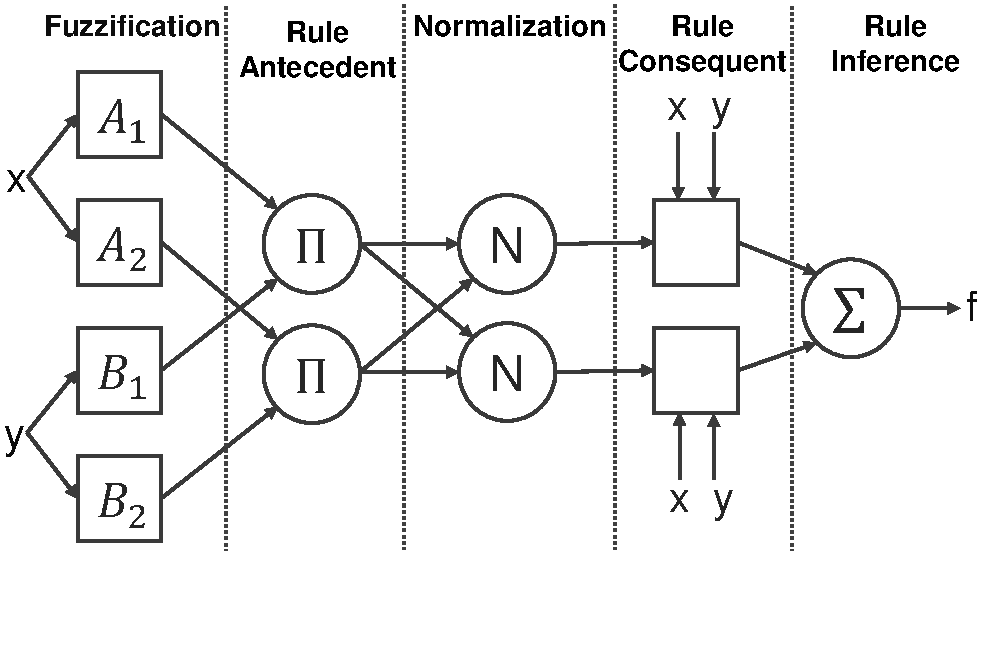
\includegraphics[width=\textwidth]{figs/Rory/ANFIS_diagram.pdf}
            \caption{}
            \label{fig:ANFIS_diagram}
          \end{subfigure}
          \hfill
          \begin{subfigure}[t]{0.48\textwidth} % Top-aligned subfigures
            \centering
            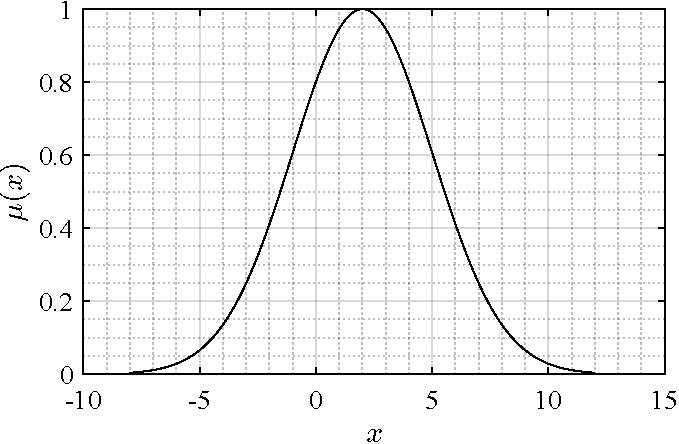
\includegraphics[width=\textwidth]{figs/Rory/mfs_plot.pdf}
            \caption{}
            \label{fig:membership_function_plot}
          \end{subfigure}
          \caption[ANFIS Network]{\textbf{a)} ANFIS network, with labelled layers. \textbf{b)} Gaussian membership function, with $c=2$ and $\sigma^2=9$.}
        \end{figure}

    
\subsection{ANFIS: Physics-Guided Fusion}

    \paragraph{Membership Functions}

        A fuzzy set is a linguistic representation of a numerical variable that has been fuzzified, enabling the modelling of uncertainty and partial truth. For example, the numerical range 1-10 can be categorised into the distinct fuzzy sets \textit{high, medium, low}. The value 9 would have a high \textit{degree of membership} in the fuzzy set \textit{high}, and a low degree of membership in the other sets. Membership functions are mathematical functions that assign each input value to a degree of membership \(\in [0,1]\) for each fuzzy set. 
        
        Gaussian membership functions have been chosen to represent the all of the environmental variables, and the sensor confidence values. The Gaussian membership function is defined as
        
        \[
        \mu(x) = \exp\left( -\frac{(x - c)^2}{2\sigma^2} \right),
        \]
        
        where \( c \) is the mode of the fuzzy set and \( \sigma^2 \) its variance, and is visualised in Figure \ref{fig:membership_function_plot}. This function is a smooth, differentiable bell curve.
        Gaussian membership functions are particularly well-suited for representing the natural variability in environmental parameters, such as soil moisture and ambient temperature, because many natural processes tend to be normally distributed, as suggested by the Central Limit Theorem \footnote{\url{https://en.wikipedia.org/wiki/Central_limit_theorem}}. Note that normalization is not necessary here because the membership values are degrees of activation rather than probability densities, and are scaled so that \(\mu(x)\in [0,1]\).
        
        In ANFIS, the network learns optimal \(c\) and \(\sigma\) parameters for each fuzzy set, tuning membership functions to best fit the fusion data. The Rule Antecedent layer determines the degree to which the fuzzy inputs satisfy the rules. The Rule Consequent layer decides the output of each rule. For Takagi-Sugeno Type-3 ANFIS \cite{jang1993anfis}, the Rule Consequents are learned as linear combinations of non-fuzzified inputs, and the outputs of all the rule consequents are combined to give a final fused confidence value. 

        
    \subsubsection{Fuzzy Rule Selection} \label{fuzzy_rules}
    

        ANFIS can be configured to include every possible 'rule' regarding the inputs to the network. However, this approach is computationally expensive, as the number of rules required scales as \((\textit{\#. fuzzy sets})^\text{(\textit{\#. inputs})}\). This makes this approach intractable when incorporating substantial domain knowledge (an example of this for time-series prediction is included in \cite{jang1993anfis}). Instead, it is more efficient to explicitly encode only the fuzzy rules that are expected to have the most significant impact, and is the approach taken here. These fuzzy rules are manually derived from the simulations in Sections \ref{compvis_thermalsims} and \ref{compvis_radarsims}, from first-principles physics, and general domain knowledge. The following rules are proposed for the ANFIS implementation:
        
        \begin{enumerate}

        
            \item \textbf{IF then soil moisture is high THEN thermal confidence is high.}\\

                \textbf{Justification:} As shown in Figure \ref{fig:conductivity}, the peak \(\Delta T\) increases with soil thermal conductivity. Given that soil thermal conductivity increases with soil water content \cite{wu2025soil}, and the \textbf{detectability hypothesis} in Section \ref{simulation_justification} argues that \(\Delta T\) can serve as a proxy for the detectability of a landmine viewed by the thermal sensor, it follows that higher soil moisture levels correlate with higher confidence in the thermal sensor.
            
            \item \textbf{IF soil moisture is high THEN radar confidence is low.}

                \textbf{Justification:} High soil moisture degrades radar performance by increasing the bulk soil electrical conductivity \cite{bai2013soils}, exponentially decreasing the penetration  depth\cite{giovanni2008penetration}, and thus reducing confidence in the radar sensor.

            \item \textbf{IF wind speed is high THEN thermal confidence is low}

                \textbf{Justification:} High wind speeds increase the rate of convective heat flux (Section \ref{compvis_thermalsims}) and tend to flatten soil surface temperature gradients, reducing \(\Delta T\) and thus reducing confidence in the thermal sensor.

            \item \textbf{IF soil is frozen THEN thermal confidence is low.}

                \textbf{Justification:} When the soil is frozen, any heat flow is absorbed by the latent heat of crystallisation, and temperature differences due to a landmine buried in the soil become undetectable. Therefore, thermal confidence is low when the soil is frozen.
 
        \end{enumerate}
        

        These rules are not exhaustive. If more domain knowledge becomes available, new fuzzy rules should be included to improve performance. To refine and expand the fuzzy rule database, an experimental campaign should be conducted to investigate the effects of additional environmental parameters on the sensor readings.

    
    \paragraph{Learning Approach of ANFIS}
    
        The ANFIS framework adopts a hybrid learning strategy that combines a feed-forward pass with backward error propagation. In the feed-forward phase, the fusion weightings (consequent parameters) are optimised with a least squares error (LSE) approach, whilst on the backwards pass, the membership function parameters (premise parameters) are optimised with gradient descent. This is described in Jang 1993 \cite{jang1993anfis}.
        
    
    By integrating physics-based constraints through fuzzy rules, and employing an adaptive learning strategy, ANFIS offers a fusion method that is both robust and interpretable. This approach is expected to outperform traditional methods by providing a solution grounded in the physical principles of sensor detection, as validated in Section \ref{compvis_anfisvalid}.
    
\subsection{ANFIS Validation} \label{compvis_anfisvalid}

Previous sections (Section \ref{fusion_bounds}) hypothesise that a physics-informed deep learning fusion network, such as ANFIS, will outperform a standard Naive Bayes (NB) fusion model. It is therefore important to validate this hypothesis with a (somewhat crude) simulation of environmental conditions and the \textbf{consequent} sensor data. This simulation aims to demonstrate that an ANFIS network with incorporated domain knowledge can improve data fusion performance over NB, when the sensor data are \textit{not} conditionally independent.

\subsubsection{Synthetic Data Generation}  
.
    ANFIS is expected to outperform NB because the latter assumes conditional independence between sensors, an assumption often invalid in real-world conditions where there is coupling between the two sensors through the causal physics of the environment. 
    
    To demonstrate NB's limitations, synthetic data is generated to model the influence of \textbf{soil moisture}. As detailed in Section \ref{fuzzy_rules}, increased soil moisture enhances thermal sensor return (via increased thermal conductivity) while inhibiting radar sensor return (via increased electrical conductivity). This is not the only coupling between the two sensors, but it suffices to model one to illustrate the advantages of ANFIS. Additionally, the model includes the effect of wind speed, which decreases thermal returns but does not affect radar returns.


    A 200$\times$200 grid was generated, with 2\% coverage of randomly placed mines. Soil moisture was simulated using a simplified sine-cosine function varying between 0 and 1, and is shown in Figure \ref{fig:anfis_summary}. Wind speed was modelled using random samples from a Gaussian distribution with a mean of 0 and a standard deviation of 2 (arbitrary units). Following the layered approach (Section \ref{layered_approach}), the radar sensor only samples points previously flagged by the thermal sensor. To simulate GPS drift and further illustrate the limitations of NB under uncertainty, a small random spatial shift was introduced between the thermal and radar datasets.


\subsubsection{Sensor Modelling}  

    The sensor confidence maps were computed using equations to model the effects of soil moisture (\textit{m}, dimensionless, ranging 0-1) and wind speed (\textit{w}, in \si{\metre\per\second}) on the thermal and radar sensor outputs. These curves are designed to reflect the higher precision characteristic of the radar sensor and the higher recall of the thermal sensor. Sensor noise was modelled as zero-mean Gaussian white noise ($\mathcal{N}$), with a variance of 0.15 for the thermal sensor, and 0.12 for the radar sensor. The resulting sensor output probabilities ($P$) are given by:
    
    \begin{equation}
        P_{\text{thermal}} = \begin{cases} 
        0.9 - 0.66e^{-m/40} - 0.02w + \mathcal{N}(0,0.15) & \text{if mine present} \\
        0.6 - 0.48e^{-m/200} - 0.02w + \mathcal{N}(0,0.15) & \text{if no mine}
        \end{cases}
    \end{equation}
    
    \begin{equation}
        P_{\text{radar}} = \begin{cases}
        1.2 \cdot 0.6e^{-m/60} + \mathcal{N}(0,0.12) & \text{if mine present} \\
        0.45 \cdot 0.6e^{-m/60} + \mathcal{N}(0,0.12) & \text{if no mine}
        \end{cases}
    \end{equation}

\subsubsection{Fusion Implementation}

    \paragraph{ANFIS} The ANFIS architecture is implemented using the Keras framework. The model accepts four input features: soil moisture, wind speed, thermal sensor confidence, and radar sensor confidence. Input fuzzification uses three Gaussian membership functions per input, whose parameters ($c,~\sigma$ in Equation \ref{eq:gaussian_mf}) are trainable variables within the network..

    While Section \ref{ANFIS} proposed explicit, physics-derived fuzzy rules, this implementation uses a \texttt{Dense} rule antecedent layer (see Figure \ref{fig:ANFIS_diagram}). A dense layer combines the membership degrees from the four inputs (each with 3 membership functions), allowing the network to learn the antecedent combinations corresponding to all $3^4=81$ possible fuzzy rules. The consequent layer learns the parameters that define the output for each of these implicitly formed rules. While traditional ANFIS employs a hybrid learning algorithm described in Section \ref{ANFIS}, this implementation utilizes standard backpropagation with the Adam optimizer for training efficiency within the Keras framework.
    
    The final custom output layer calculates a normalised, weighted sum of these rule outputs and applies a sigmoid function to ensure the final fused confidence is between 0 and 1.

    \paragraph{NB} The Naive Bayes (NB) fusion method combines the thermal and radar sensor confidence values $P_{\text{thermal}}$, $P_{\text{radar}}$. Assuming conditional independence between the sensors given the presence or absence of a mine, the fused confidence $P_{\text{fused}}$ is calculated using Bayes Theorem, which may be written as:

    \begin{equation}
        \label{eq:bayes_fusion}
        \mathcal{P}_\text{fused} = \frac{\mathcal{P}_\text{thermal}\mathcal{P}_\text{radar}}{\mathcal{P}_\text{thermal}\mathcal{P}_\text{radar} + (1-\mathcal{P}_\text{thermal})(1-\mathcal{P}_\text{radar})}
    \end{equation}
    
\subsubsection{Results and Conclusion}  

    The ANFIS model demonstrated improved recall (ANFIS: 0.66 NB: 0.11) and precision (ANFIS: 0.92 NB: 0.28), compared to Naive Bayes. The surprisingly low NB performance is partly caused by the random shifting between the radar the thermal maps, that means NB often gives null results from multiplying misaligned confidence values. However, more fundamentally, the simulation highlights ANFIS' key advantage; it can leverage the environmental context (soil moisture and wind speed inputs in this implementation) to implicitly model the physical coupling between sensor readings. Naive Bayes' inability to handle uncertainty and conditionally dependent data is also clear. See the predicted mine locations from each fusion algorithm in Figure \ref{fig:anfis_summary}.

     While this simulation is simplified, it validates the hypothesis that a deep learning fusion architecture, constrained to physically-plausible solutions and incorporates environmental context can perform significantly better than purely statistical methods, like Naive Bayes.

    \begin{figure}[h]
        \centering
        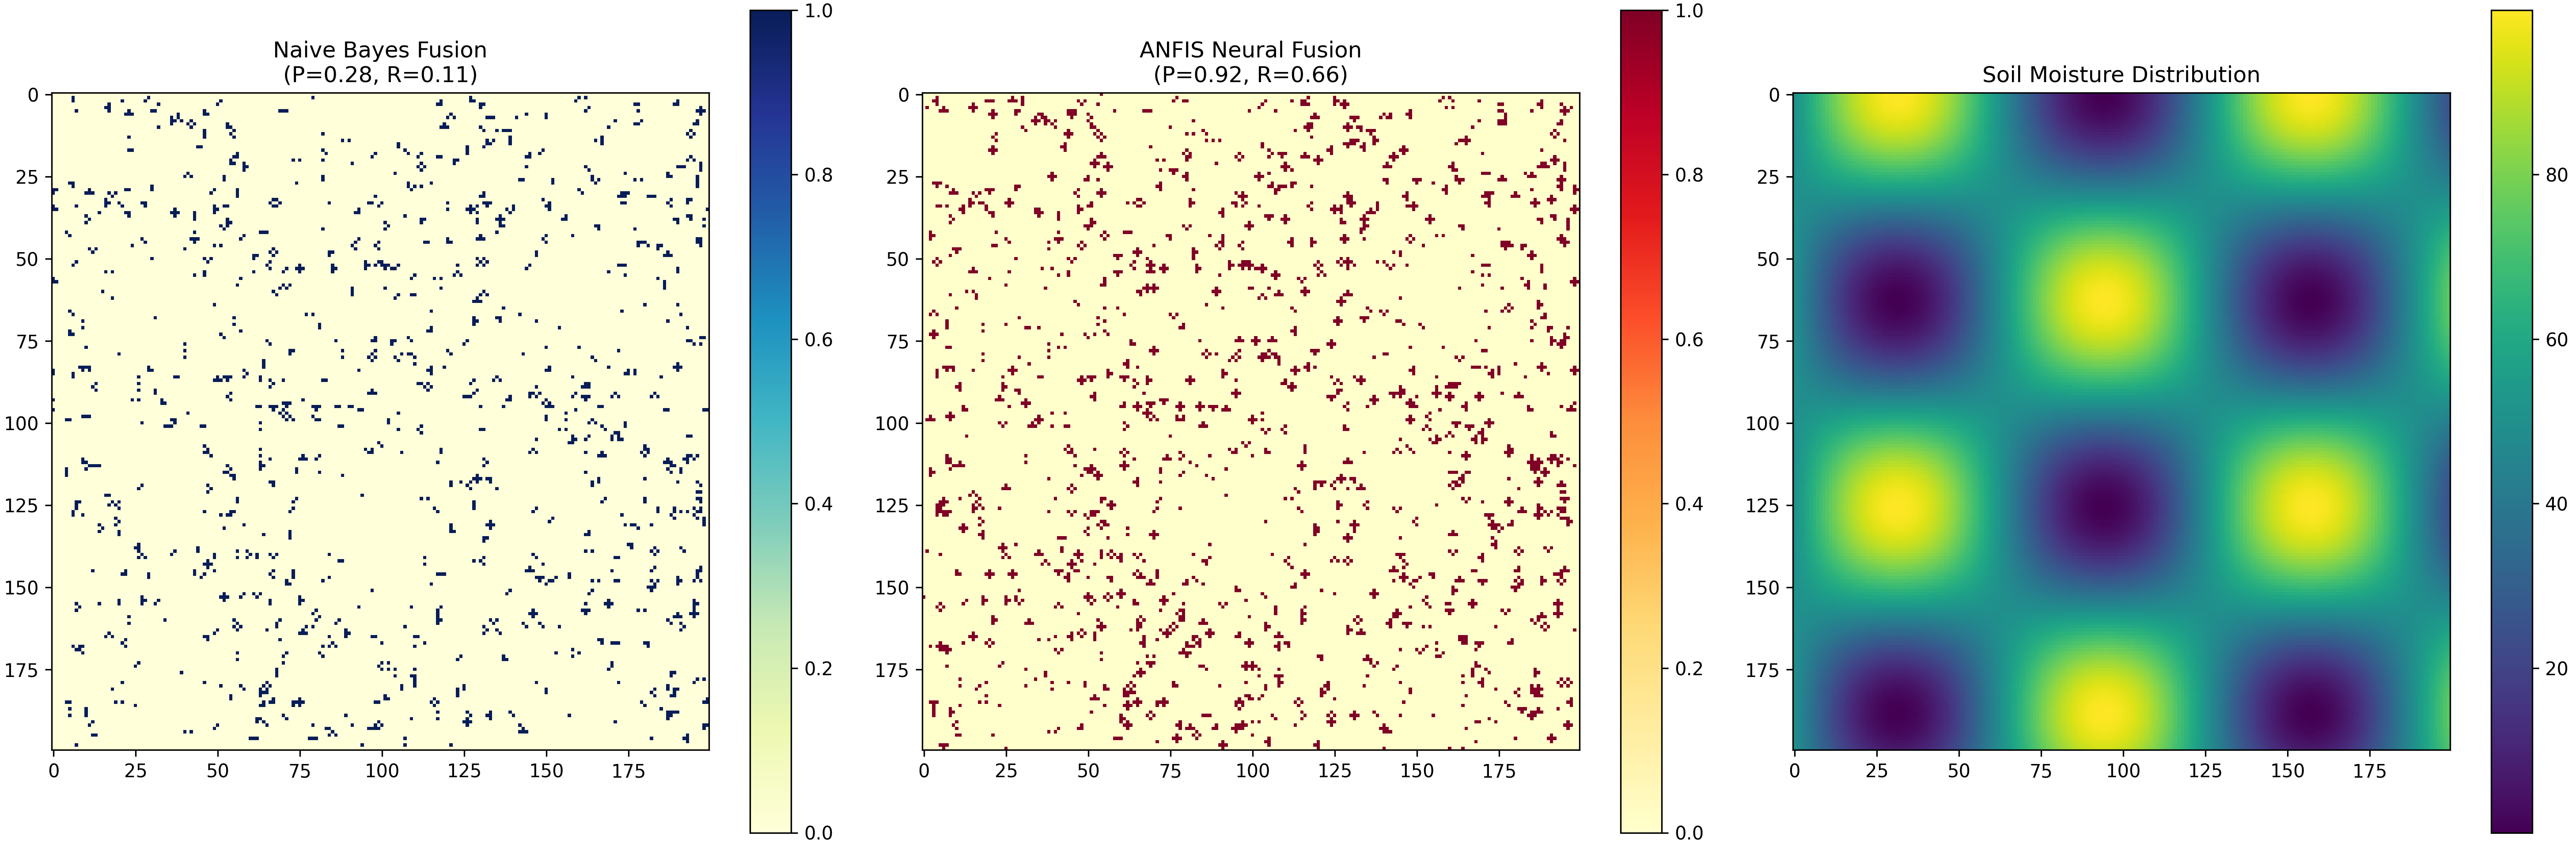
\includegraphics[width=0.98\textwidth]{figs/Rory/0_summary.png}
        \caption{ANFIS NB comparison summary. \textbf{Left:} simulated fusion for Naive Bayes. \textbf{Centre:} simulated fusion for ANFIS. \textbf{Right:} soil moisture distribution}
        \label{fig:anfis_summary}
    \end{figure}

    \paragraph{Future Work} 

        Several other physics-driven fusion algorithms exist. Another such approach is \textit{Physics Based Deep Learning} (PBDL)\footnote{\url{https://www.physicsbaseddeeplearning.org/intro.html}}, which benefits from implementing the physical domain knowledge at a deeper level in the \textit{model architecture and loss function}. PBDL is a recent field in Artificial Intelligence (AI), and it may have significant benefits, such as greater robustness to environmental variations in data-fusion for the detection of landmines.




\newpage
\fancyhead[C]{Samuel Grace}
\section{Simulation and Control} \label{simulationandcontrol}

Samuel Grace 123 \cite{cabreira2019cpp}

\newpage
\fancyhead[C]{Thomas Turner}
\section{Intra-UAV Communication Architecture} \label{Intra Communication}

\subsection{Introduction and Philosophy}
The communication and networking of devices on our device is a key consideration for design. This is because of the specific design challenges of achieving redundancy and modularity at low power and low cost. In line with these key design guidelines all interfaces and software should be as uniform as possible to reduce the training required for operation and to reduce the difficulty of creating new components for specific environments and regulations.


\subsection{Design Considerations}\label{sub_sub_section:tgt_intra_comms_design_considerations}

\subsubsection{Modularity}\label{sub_sub_section:tgt_modularity}
\paragraph{Relevance}
Mechanical modularity is the most obvious path as the components need to physically connect easily. However, the communication architecture also needs to support this so that devices can easily communicate even if they are changed completely.
\paragraph{Modular Communication Protocols}
Defined interfaces, protocols and pin allow for different devices to communicate without specific dependencies on each other. Therefore, integrating new sensors or modules does not require a new communication system. Another key property of modular networks is physical, some networks lend themselves better to modular design, for example for a \gls{CAN} FD Bus you only need to add a stub and all interfaces should use standard connectors.

\subsubsection{Telemetry}\label{sub_sub_section:tgt_telemetry}
\paragraph{Battery Telemetry}
The two key failure modes for the battery are state of charge and thermal runaway. Both can cause complete failure and therefore both should be monitored during flight. This allows for \gls{RTH} to be triggered in case of a state of charge or emergency landing in the case of thermal runaway. Therefore, real-time telemetry is sent from the \gls{BMS} to the flight controller for temperature and state of charge.
\paragraph{\gls{ESC} Telemetry}
Providing \gls{ESC} telemetry for voltage, current and \gls{RPM} is important information when classifying motor and propeller faults accurately which is needed to support the adaptive control strategy in Section \ref{sub_sub_section:tgt_actuator_fault}. Furthermore, \gls{ESC} temperature is also sent to monitor for overheating. 

\subsubsection{Communication Bus}\label{sub_sub_section:tgt_bus}
\paragraph{\gls{CAN} bus}
In order to support the \gls{ESC} telemetry required Cyphal should be used as it is widely supported by \gls{COTS} hardware and can run over \gls{CAN} bus. CAN Flexible Data (FD) is widely used and supported and can process data transfer speeds up to 8 Mbps using the transceiver used in Section \ref{section:Custom Hardware}\footnote{\url{https://www.ti.com/lit/ds/symlink/tcan1472-q1.pdf}} whilst also supporting modularity. In order to guarantee redundancy a dual \gls{CAN} bus is selected so if there is a failure on one bus, the other bus is used. Failures can be detected across the bus as all modules will communicate 10 Hz heartbeats to each other indicating that they are operating as normal so if this heartbeat is not received the redundant bus is used instead. This allows for failure handovers in just 0.1s. Lastly, as \gls{CAN} is a differential signal the lines are carried in a twisted pair and transferred in a sheaf to reduce \gls{EMI} and risk of damage. 
\paragraph{Imaging Separation}
The images used in GPR and Thermal require significantly more data then both telemetry and command signals. Therefore, they are separately connected to the on-board computer using 1000BASE-T Gigabit Ethernet supporting data transfer speeds up to 1 Gbps. It also utilises a copper twisted pair and differential signal for noise rejection \cite{Ethernet}.  This supports thermal and GPR imaging in addition to future upgrades and increased data transfer rates.
\paragraph{Node Distribution}
Safety critical devices ensure that the drone does not sustain damage or isolate itself. This includes components necessary for flight and the sensors required for \gls{RTS} explored in Section \ref{Return to Safety}. To ensure that failures are minimised, safety critical devices should be redundant. If a safety critical device does not have a redundant version it should be able to communicate on at least two different lines preventing a single module failure causing device failure. Distributing the devices on different communication lines reduces the risk of failure as it reduces the risk of common mode failure. For example, if a \gls{GNSS} module were to have an improper fixture and move in a way that it severs all connections; if both communication lines are in it, both are severed. However, if it is on only one communication line then the other communication line is undamaged. This layout is shown in Figure \ref{fig:CAN_bus}. 
 \begin{figure}[h]
 \centering
  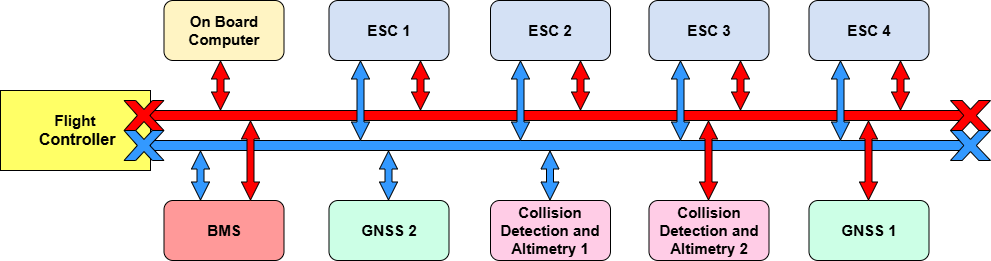
\includegraphics[width=1\textwidth]{figs/Thomas/Intra Communication/CAN bus.png}
 \caption{Bus layout}
 \label{fig:CAN_bus}
 \end{figure}
\paragraph{Communication Architecture}
Centralised architectures consist of a central node directly connected to all the relevant devices. while this is a simple and cost effective method it leaves the device to single points of failure. In order to build robustness, the custom \gls{GNSS} module is capable of independently executing landing and \gls{RTS} as it is equipped with an independent \gls{IMU} that is control capable. The \gls{GNSS} module sends control signals if the flight controller is no longer received ensuring smooth handover. 
\paragraph{High Level Protocol}
A single high level protocol being used across all components makes the \gls{UAV} more adaptable and makes hiring developers easier. This is because a single skill-set can interact with the entire system. Therefore, Cyphal will be used as it can operate over \gls{CAN} and Ethernet which are the key communication systems. It is used over alternative application protocols including ROS 2 and Mavlink as it has wider support from \gls{COTS} \gls{ESC}s\footnote{\url{https://opencyphal.org/}} . 
\subsection{Protocol Selection}\label{sub_section:tgt_protocol_selection}

\subsubsection{Requirements and Options}\label{sub_sub_section:tgt_requirements}
\paragraph{Message Requirements}
Table \ref{tab:messages} shows the required messages for flight and imaging. From this it is clear that imaging requires a far higher data transfer speeds. This means a network of low speed modules could be used with a separate imaging network.
\begin{table}[h]
\centering
\begin{tabular}{|c|c|c|c|c|c|c|} 
\hline
\textbf{Protocol} & \textbf{Speed} & \textbf{Complexity} & \textbf{Power Draw} & \textbf{Noise Tolerance} & \textbf{Cost} & \textbf{Use Case} \\ 
\hline 
CAN FD & 5 Mbps & Medium & Medium & High & Medium & Bus \\ 
FlexRay & 10 Mbps & High & High & High & High & Bus \\ 
I$^2$C & 400 Kbps & Low & Low & Low & Low & Sensors \\ 
SPI & 100 Mbps & Medium & Low & Medium & Low & Sensors \\ 
UART & 1 Mbps & Low & Low & Low & Low & Sensors \\ 
Ethernet & 1 Gbps & Medium & Medium & High & Medium & Imaging \\ 
\hline 
\end{tabular}
\caption{Communication Protocols}
\label{tab:communication_options}
\end{table}
\begin{table}[h]
\centering
\begin{tabular}{|c|c|c|c|c|} 
\hline
\textbf{Purpose}&\textbf{Frequency (Hz)}&\textbf{Message Size(bits)}&\textbf{Quantity}&\textbf{Bandwidth (kbps)}\\
\hline
ESC Duty Cycle&400&16&4&25.6\\
ESC Telemetry&10&64&4&2.56\\
Fault ESC Telemetry&400&64&4&102.4\\
Imaging Location&100&48&1&4.8\\
BMS Telemetry&10&32&1&0.32\\
GNSS location&10&48&2&0.96\\
Collision Detection&100&16&2&3.2\\
GNSS Correction&1&500&1&0.5\\
\hline
\end{tabular}
\caption{Required Standard Messages}
\label{tab:device_comms_requirementsl}
\end{table}



\subsubsection{Communication between Modules}\label{sub_sub_section:tgt_comms_modules}
\paragraph{Architecture}
Centralised architectures consist of a central node directly connected to all the relevant devices, creating a single point of failure. while this is a simple and cost effective method it leaves the device to single points of failure. In order to build robustness, the custom \gls{GNSS} module is capable of independently executing landing and \gls{RTS}.  
\paragraph{Bus Selection}
FlexRay has some clear advantages including built in redundancy and higher data transfer speeds as shown in Table \ref{tab:communication_options}. However, due to its added complexity, cost and the fact it is compatible with far fewer components, a \gls{CAN} bus is the better option. This may change if the data transfer rates needed to increase or if the technology behind FlexRay becomes cheaper and more widespread. Further, there are two key options for \gls{CAN}, time triggered or flexible data. Time triggered is an attractive as it supports higher data transfer rates however, flexible data is more widely supported and is sufficient for the application.\cite{CANFlexRay}
 
\subsubsection{Communication with sensors}\label{sub_sub_section:tgt_comms_sensors}
\paragraph{High Speed Sensors}
The simple but high speed \gls{SPI} protocol should be used whenever possible. This is because it is widely supporting by commercially available sensors and \gls{MCU}s. Uniformly using similar sensor sets also has the benefit of simplicity of implementation.
\paragraph{Low Speed Sensors}
Both \gls{UART} and \gls{I$^2$C} are widely supported, both are simple and effective however, \gls{UART} is slightly wider supported therefore on non-complex modules is used where possible. However, if pins are limited \gls{I$^2$C} should be used as it can bus multiple low speed sensors.
\paragraph{Memory Devices}
MicroSD and SD cards can communicate with \gls{SPI} or \gls{SDIO}. \gls{SPI} uses 1 bit writing and \gls{SDIO} uses 4 bit communication making \gls{SDIO} faster but harder to design traces with\footnote{\url{https://fmuser.org/news/IPTV-encoder/Introduction-to-SPI-I2C-UART-I2S-GPIO-SDIO-CAN/}}. Therefore, for the flight controller \gls{SPI} was used as the data transfer rates are low. However, while recording imaging data on the main computers SD card, \gls{SDIO} should be used in order to support the high writing speeds required. 
\paragraph{Imaging Sensors}
The imaging sensors require very high data transfer rates of over 34 mbps and are not safety critical. They are therefore not included on the \gls{CAN} bus but instead directly connect to the onboard computer using Ethernet as it can handle the higher speeds required.
\paragraph{Debugger}
Debugging is possible using the \gls{CAN} bus at a system level but for in depth on board debugging that might be required for failure analysis or uploading code to boards should also be available.\gls{UART} can be used as a live signal monitor similar to CAN however, for full access debugging a \gls{SWD} interface is used\footnote{\url{https://runtimerec.com/using-debugging-interfaces-uart-jtag-and-swd-demystified}}. Therefore, for system wide debugging the \gls{CAN} bus will be used, and for onboard debugging a \gls{SWD} will be used.
\paragraph{High Level Protocol}
A single high level protocol being used across all components makes the \gls{UAV} more adaptable and makes hiring developers easier. This is because a single skill-set can interact with the entire system. Therefore, Cyphal will be used as it can operate over \gls{CAN} and Ethernet \footnote{\url{https://opencyphal.org/}} which are the key communication systems. 

\newpage
\fancyhead[C]{Thomas Turner}
\section{Custom Hardware} \label{section:Custom Hardware}
\subsection{Introduction and Philosophy}
Due to the specific operating environment, custom hardware is required. This is because the device cannot safely carry out emergency landing procedures when a fault is detected due to the difficulty of retrieval. Furthermore, any crashes can damage the onboard imaging sensors. Lastly, there is significant opportunity cost of delaying mapping as the equipment and manpower involved in demining would be ineffective until retrieval and repair or replacement of the device. 
\paragraph{When to use custom components}
\gls{COTS} options should always be considered before any custom part due to the significant design and testing costs associated with custom parts. Furthermore, \gls{COTS} options will often have shorter lead times and will benefit from sourcing at greater scales. However, when there are specific design requirements not met in the current market custom components need to be used.
\paragraph{Objectives}
All hardware should be easy and quick to debug, it should support redundancy and it should be as modular as possible. Furthermore, they should also line up with our sustainability and inclusion objectives by ensuring all components are \gls{RoHS} compliant and, where applicable, should support those with disabilities. I will design core components demonstrating the design principles explored however, not all hardware components are considered and there is significant room for future work.

\begin{figure}[htbp]
 % Row 2: Legend + GNSS Gerber and Render
  \centering
  \begin{subfigure}[b]{0.48\textwidth}
    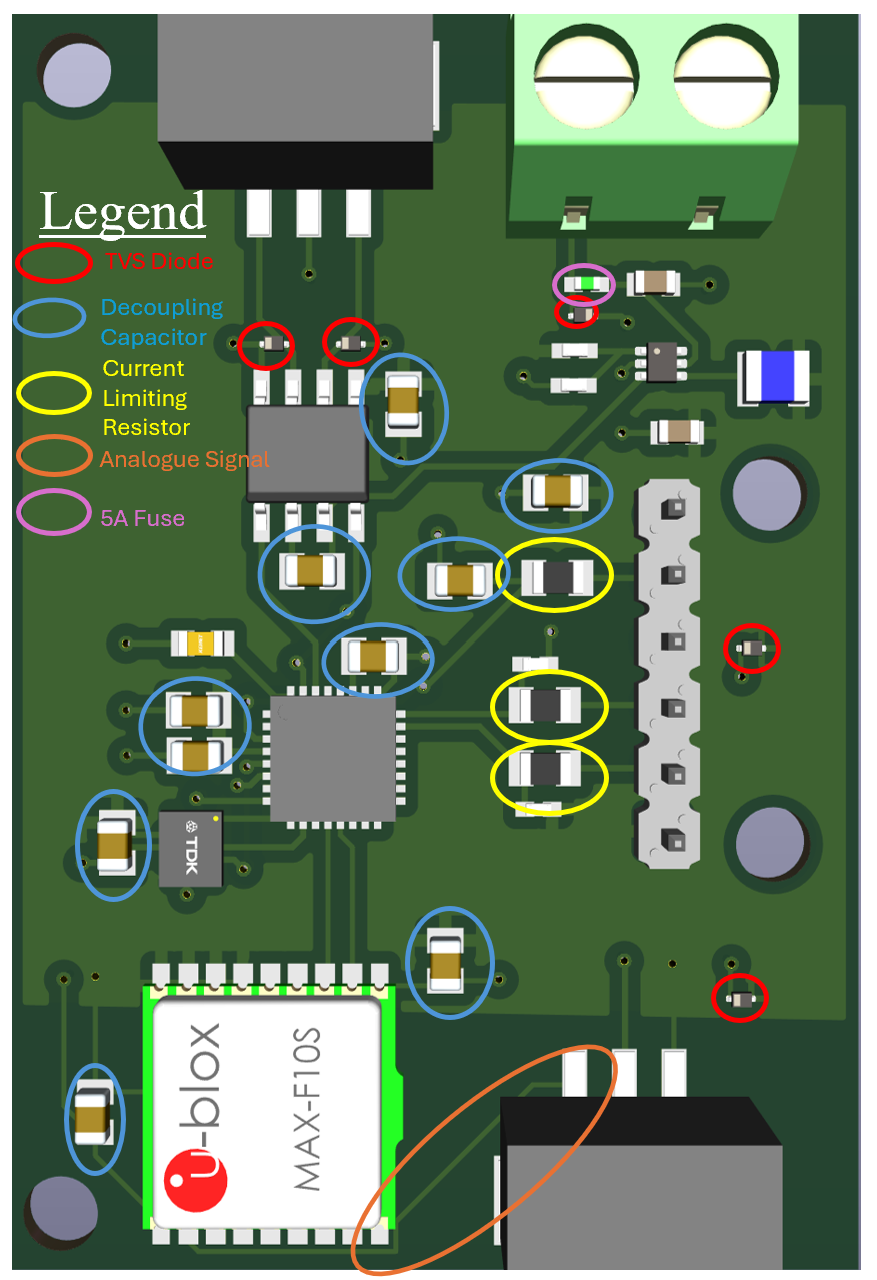
\includegraphics[width=\textwidth]{figs/Thomas/Custom Hardware/GPS render.png}
    \caption{GNSS Module Render}
    \label{fig:gnss_render}
  \end{subfigure}
  \hfill
  \begin{subfigure}[b]{0.48\textwidth}
    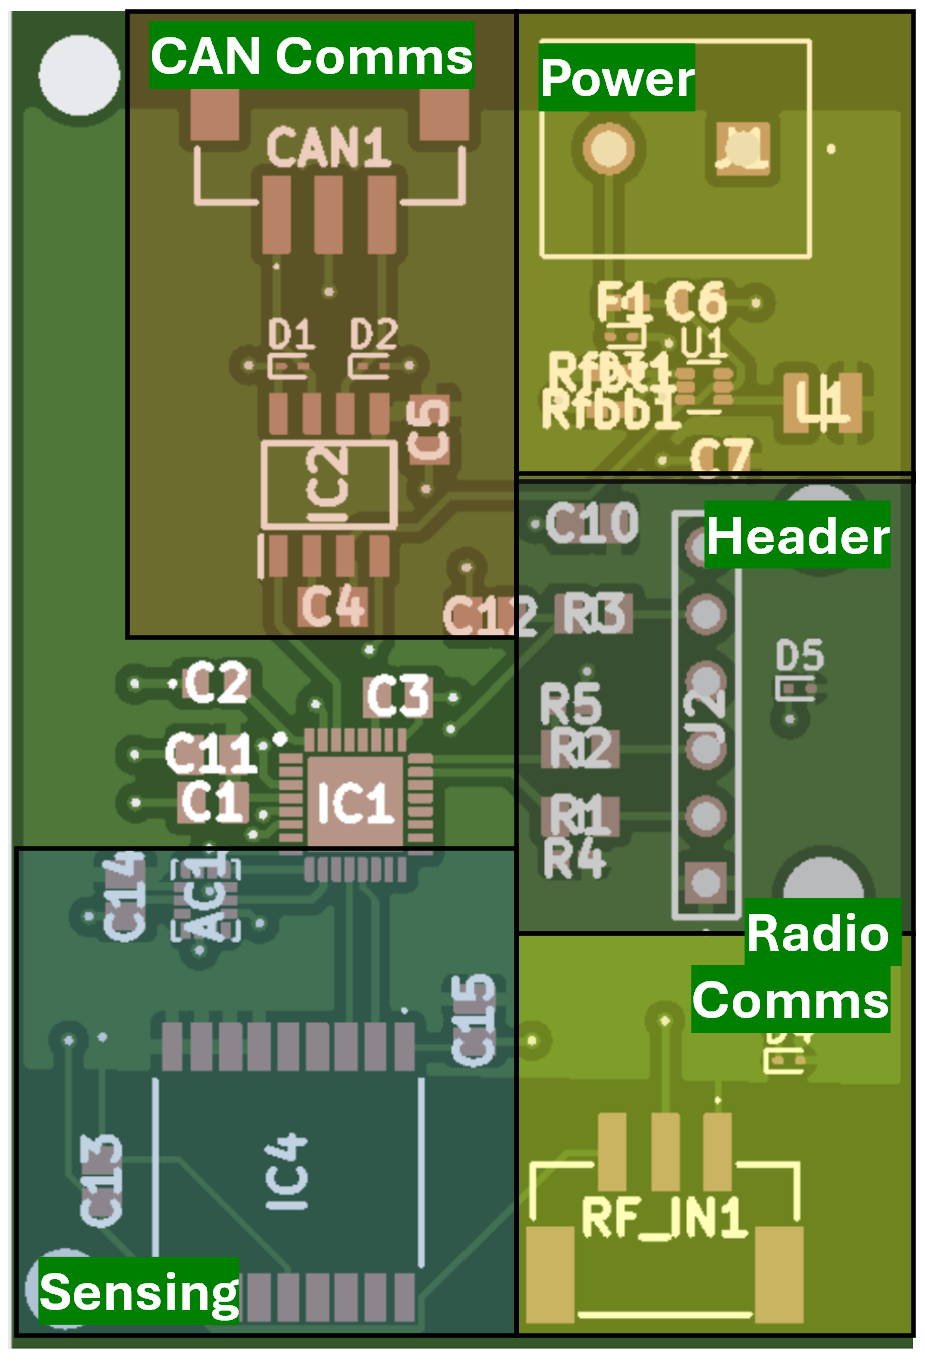
\includegraphics[width=\textwidth]{figs/Thomas/Custom Hardware/GPS gerber.png}
    \caption{GNSS Module Gerber}
    \label{fig:gnss_gerber}
  \end{subfigure}

  
  \begin{subfigure}[b]{0.48\textwidth}
    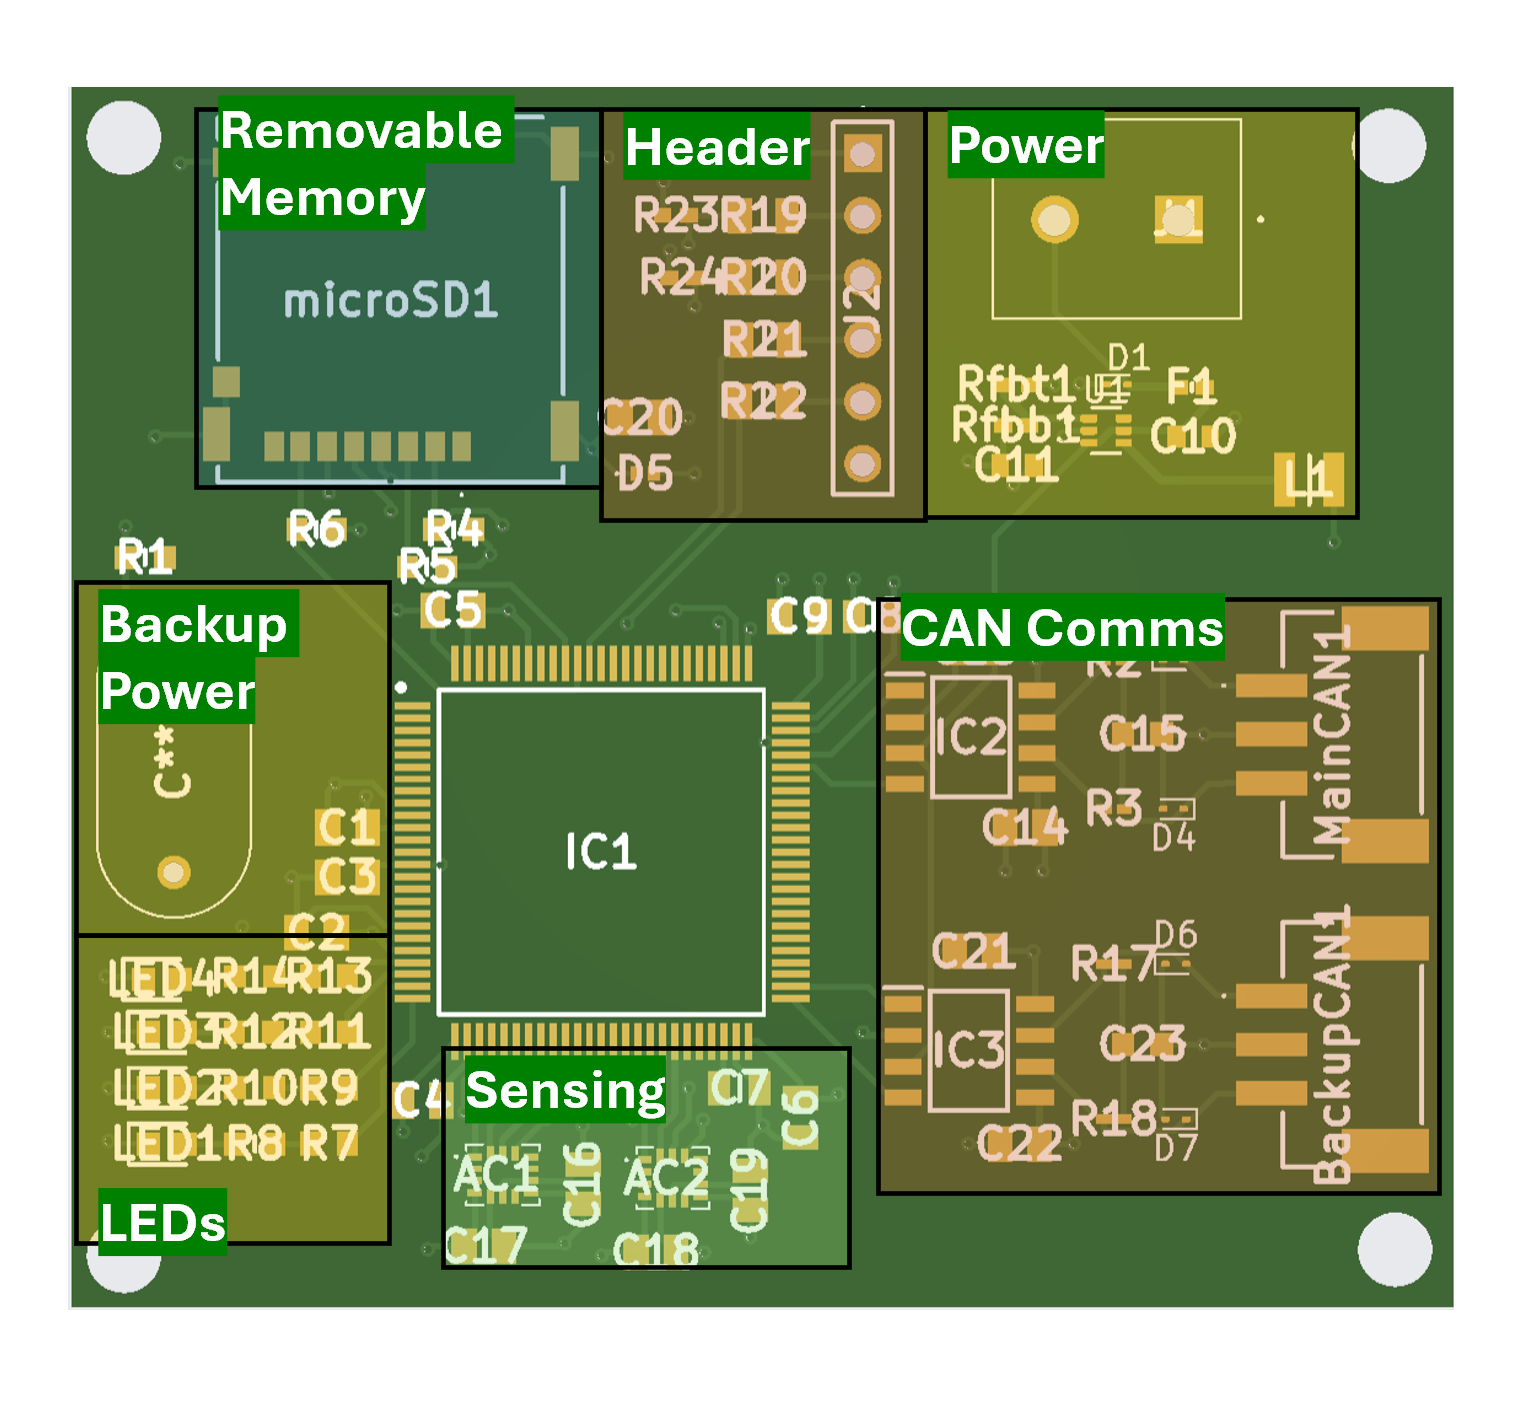
\includegraphics[width=\textwidth]{figs/Thomas/Custom Hardware/FC gerber.png}
    \caption{Custom Flight Controller Gerber}
    \label{fig:fc_gerber}
  \end{subfigure}
  \hfill
  \begin{subfigure}[b]{0.48\textwidth}
    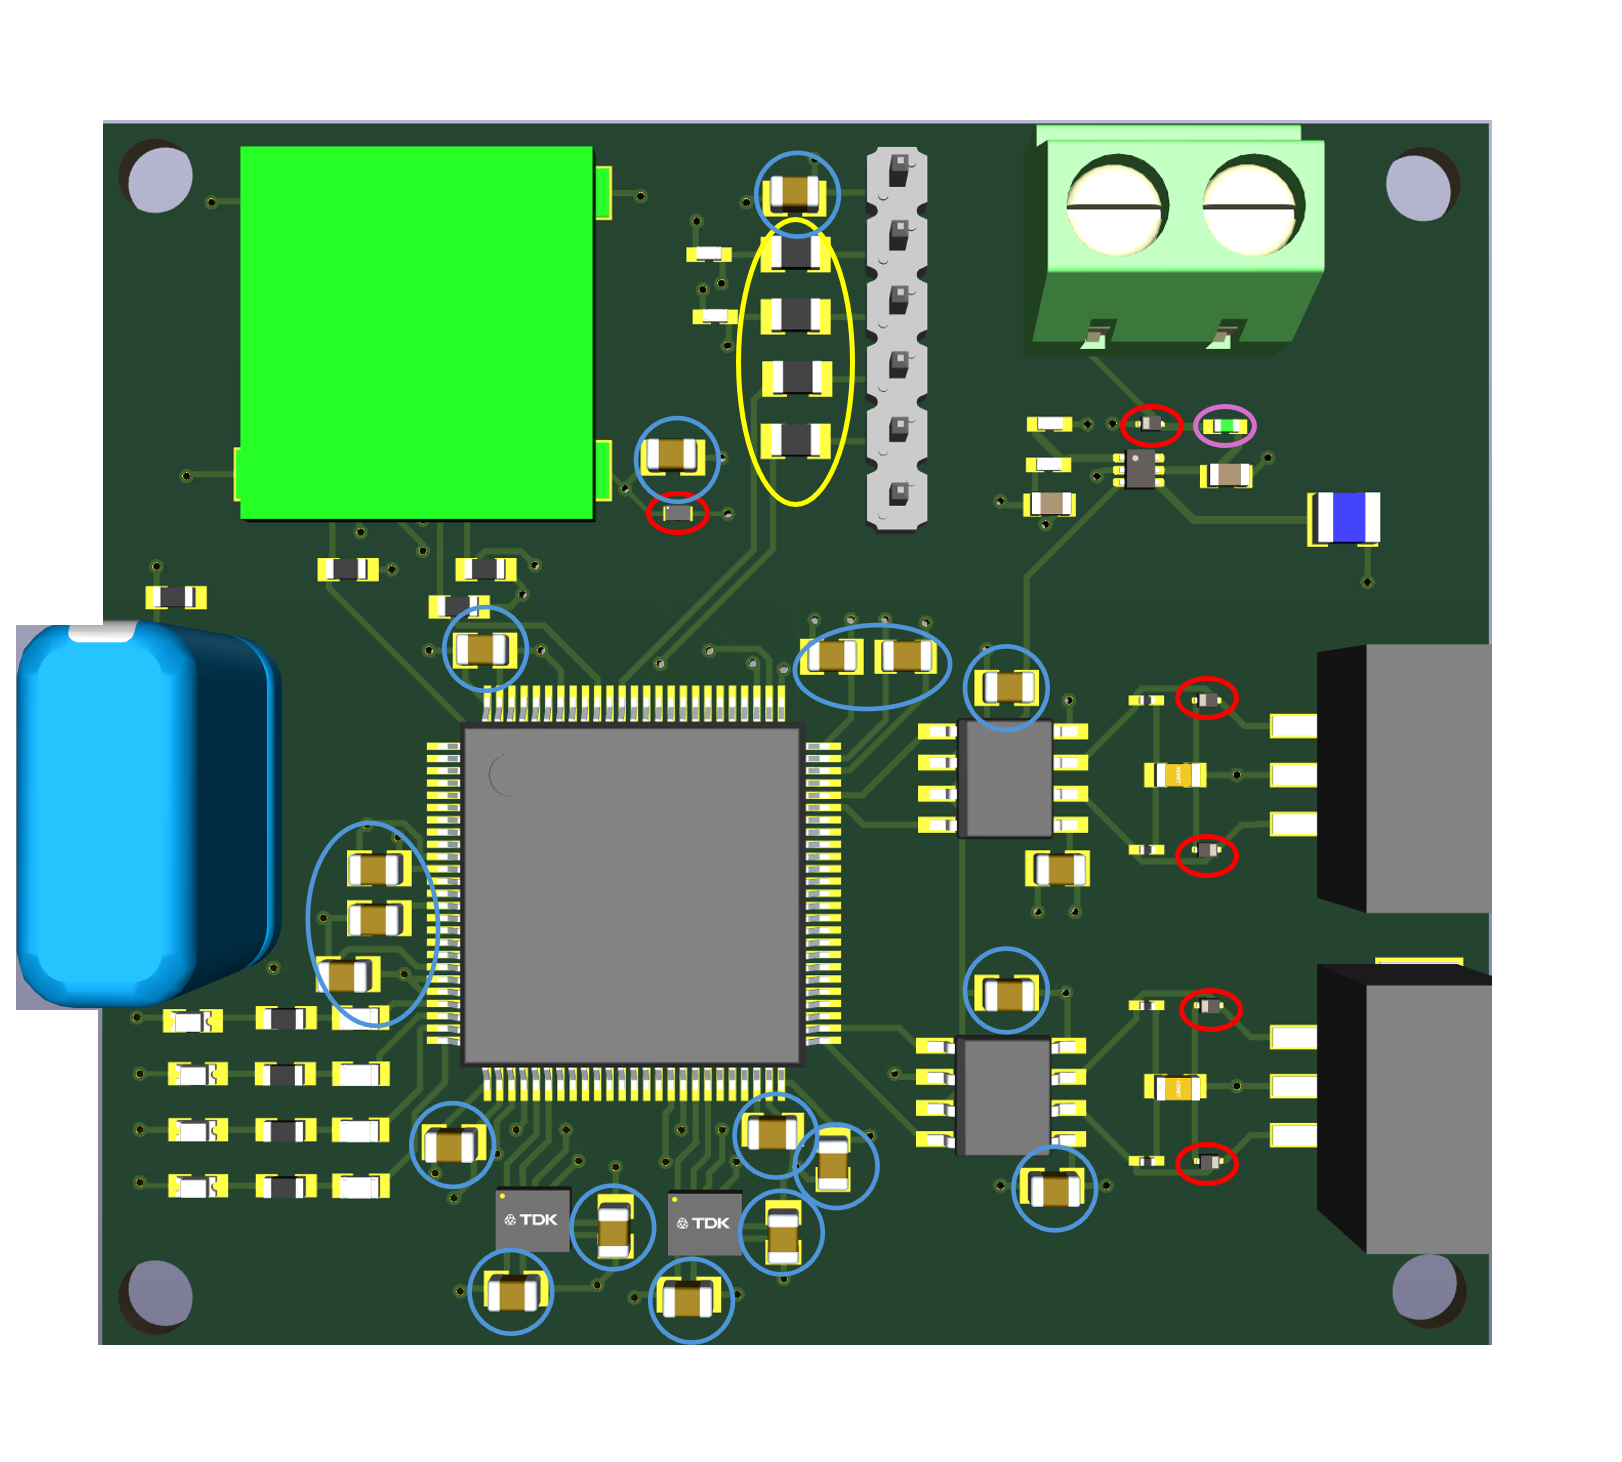
\includegraphics[width=\textwidth]{figs/Thomas/Custom Hardware/FC render.png}
    \caption{Custom Flight Controller Render}
    \label{fig:fc_render}
  \end{subfigure}

  \vspace{1em} % space between rows
  \caption{Custom Hardware Boards: Flight Controller and GNSS Module with Legend}
  \label{fig:custom_hardware_overview}
\end{figure}

\subsection{Design Considerations}

\subsubsection{Trace Lengths}
\paragraph{Signal Integrity and Timing}
All traces have propagation delay that increases linearly with length \cite{REF} meaning that the longer the trace, the longer the delay. Furthermore, noise increases due to impurities and crosstalk. Therefore, traces should be kept as short as possible. This means that large footprint devices are placed at the edges and the \gls{MCU} is placed centrally.
\paragraph{Length Matching}
In synchronous communication methods the clock signal must be in sync with the data transmission. This means that the lines should be as similar in length as possible so that they arrive at the same delay. The faster the communication rate the stricter this must become as the clock signal frequency is increased \cite{REF}.
\paragraph{Effect of vias}
Vias allow for the transference of signals between planes which is necessary for routing signals. However, they should be avoided as they introduce extra impedance, noise and delay. Furthermore, for synchronous high speed signals they should be included in trace length considerations as the line with fewer vias should be tuned to have a longer length to achieve the same delay.

\subsubsection{Protection}
\paragraph{\gls{ESD}}
\gls{ESD} occurs when there is a significant static charge built up in a ground operator or contacting surface that is then shorted in contact with the board. As electro-static voltages can be xxV \cite{REF} this can cause significant damage to devices due to transient current spikes.
\paragraph{Touch Protection Devices}
In order to protect against \gls{ESD} the circuit must provide a low resistance pathway to the ground. This can be using \gls{TVS} diodes that above certain voltages act like a wire that diverts the current flow. They can also be mitigated using voltage dependent resistors that increase resistance with voltage, preventing current spikes. In my designs I make use of bidirectional \gls{TVS} diodes due to their price and simplicity. 
\paragraph{Over current protection}
Fuses and resistors are the best way to protect a device against short circuits. Series resistors mitigate the peak current therefore, for serial debugging I ensured that all connections direct to the \gls{MCU} have series resistors in case of accidental short circuits by the user. However, fuses are the best way to protect against short circuits. This is because, series resistors dissipate too much power to be efficient in power transfer lines, therefore 5A fuses are used in the power lines of both modules. 
\paragraph{Placement}
Protections should be as close to possible sources so the least number of components and wires get damaged in failure. Therefore, all \gls{TVS} diodes are placed near touched areas or interfaces, series resistors are placed as close as possible to prevent wire transients and fuses are placed before the power is connected to the power and ground planes.

\subsubsection{Component Placement}
\paragraph{Utility Regions}
Components with similar functionalities should be restricted to specific regions, this is because it reduces trace length, prevents interference between high and low frequency signals and makes thermal management easier. These regions for the custom designed hardware can be seen in\ref{fig:custom_hardware_overview}.
\paragraph{Thermal Considerations}
Heat dissipating elements, typically diodes and resistors, can cause damage to electronic component, therefore, heat sinks or controlled airflows are sometimes required. This consideration is why on my devices Buck Converters of above 90\% are used instead of the less efficient \gls{LDO} which would have an efficiency of 66\% when converting from 5V to 3.3V. This, in addition to the low power draws of all other components, means that no explicit thermal management is needed.

\subsubsection{Trace Widths and Spacing}
\paragraph{Impedance Control}
The impedance of a trace in inverse proportion to its cross sectional area as it acts like a wire \cite{a source}. Since the trace thickness standard as one ounce per square foot \cite{source} it is the cheapest to manufacture with and is used. Therefore, to control the impedance of a trace the width must be calibrated. \textbf{a nice table showing the widths and current capacities and specific operations}
\paragraph{Crosstalk}
When traces are too close too each other they can induce signals in each other \cite{REF}. However, since all the signals are digital or physically isolated on the board this is not a major concern but I did ensure that all traces are at least 1.5 trace widths separated as a form of best practice. Furthermore, the Radio Frequency input for the \gls{GNSS} module is kept away from all other components and the ground and voltage planes as shown in \ref{fig:gnss_render}).

\subsubsection{Layers}
\paragraph{Two Layers}
The simplest and most cost effective option in \gls{PCB} design is two copper layers separated by a dielectric \cite{REF}. By using a copper filled regions you can create a ground plane and a power plane that effectively distribute charge and maintain voltage integrity. The simplicity of the \gls{GNSS} module means that two layers is the best option. This comes at the cost of more difficult component placement and a slightly less stable power and ground plane. To mitigate the instability, distributed ceramic capacitors between the planes that filter high frequency noise in voltage levels, maintaining integrity. These capacitors are best placed next to sensors and processers to ensure stable, low noise readings.
\paragraph{Four or More Layers}
When circuits become more complex, a purpose ground and power plane in between the top and bottom plane can allow for greater packing density of components. They also make the planes more stable as all the path impedances are very low. This means that for complex designs with many sensors, like the flight controller module, four layer \gls{PCB}s are the best option. Furthermore, if the complexity of the design is greater you can add further ground and power planes for analogue signals, high frequency signals or for regular signals to support greater component density.

\subsection{Debugging}
\paragraph{Technical Debugging}
There easy to use male pin headers in both designs shown in \ref{fig:custom_hardware_overview} so that a \gls{SWD} debugger can be connected, furthermore, for signalling debugging the detachable ports for the \gls{CAN} bus mean a debugging computer can simply connect. This is so technically skilled operators can inspect system level signals and specific board operations.
\paragraph{Field Debugging}
The use of technical debugging experts should always be avoided if possible to reduce capital expenditure and delay. Therefore the custom flight controller has a simple 4 \gls{LED} array for basic error codes that can isolate the problem so it can be fixed or so that only a specific, replaceable component, can be sent for repair and switched out with a backup. These codes are shown in \ref{tab:error_codes} where the colours are the \gls{LED}s and the x denotes blinking, the null state is a solid green \gls{LED} only.  The inclusion of the green LED has three key purposes: firstly, it blinks to denote between modules, secondly it gives clear visualisation that no tests have failed and lastly it ensures the codes are red in the right order no matter the orientation. It is also a different brightness to the red \gls{LED}s allowing for use by colour-blind operators in line with the inclusion objectives of the project.
\begin{table}
\centering
\begin{tabular}{|l|c|l|c|l|c|l|c|}
\hline
\textbf{Failure} & \textbf{Code} & \textbf{Failure} & \textbf{Code}& \textbf{Failure} & \textbf{Code} & \textbf{Failure} & \textbf{Code} \\
\hline
CAN 1 & \drawcode{white}{red}{red}{red} & CAN 2 & \drawcode{blinkgreen}{red}{red}{red} &
GNSS 1 & \drawcode{white}{red}{red}{white} & GNSS 2 & \drawcode{blinkgreen}{red}{red}{white}\\

Flight Controller & \drawcode{white}{red}{white}{white} & BMS & \drawcode{blinkgreen}{red}{white}{white} &
Collision 1 & \drawcode{white}{white}{red}{white} & Collision 2 & \drawcode{blinkgreen}{white}{red}{white}\\

ESC 1 & \drawcode{white}{blinkred}{blinkred}{blinkred} & ESC 2 & \drawcode{white}{red}{blinkred}{blinkred} &
ESC 3 & \drawcode{white}{red}{red}{blinkred} & ESC 4 & \drawcode{white}{red}{blinkred}{red}\\

Altimetry 1 & \drawcode{white}{white}{white}{red} & Altimetry 2 & \drawcode{blinkgreen}{white}{white}{red} &
LoRa & \drawcode{white}{white}{red}{red} & Unknown & \drawcode{blinkgreen}{blinkred}{blinkred}{blinkred}\\
\hline
\end{tabular}
\caption{Flight Controller LED Error Codes}
\label{tab:error_codes}
\end{table}
\paragraph{Post Failure Analysis}
If there is a crash that causes significant damage, and due to the volatile nature of \gls{RAM} memory, some failures cannot be detected directly with the device. Therefore, the flight controller has a removable microSD card to record flight data. In addition, the backup power supply, as seen in \ref{fig:custom_hardware_overview}, provides enough power that even in complete failure it can write the final few error messages. Therefore, this can be retrieved, downloaded and sent for analysis quickly to find the source of failure.
\subsection{Custom Components}\label{sub_sub_section:tgt_custom_components}

\subsubsection{Component Selection}\label{sub_sub_section:tgt_component_selection}


\paragraph{\gls{IMU}}
While the BMI323 is cheaper it has higher noise characteristics than the the ICM-42688-P, therefore the latter was selected for use on all boards due to its low price point and high performance. The use of the same \gls{IMU} over all modules should be maintained if possible so that the control characteristics are unchanged across devices and lower costs due to higher order quantities.
\paragraph{\gls{MCU}}
For the flight controller the STM32H743VGT6 is the best option given its \gls{RAM}, price point and support of dual \gls{CAN} buses. However, for the less computationally intense operations required for the \gls{GNSS} module the smaller footprint (due to the lower number of pins) and lower priced MSPM0G3506SRHBR is a better option.
\paragraph{\gls{GNSS} Module}
Exact positions for where the images were taken to cm precision is required as discussed in Section \ref{GPR_design}, this is possible using a \gls{RTK} setup with a base station sending out correction vectors over LoRA getting within cm accuracy\cite{RTK_LORA}. Furthermore, in the case of the loss of all \gls{GNSS} signal built in dead reckoning, allowing \gls{RTS}, is also a desirable feature. Therefore, the LG69T-AP is selected. However, when not executing imaging tasks, this precision is not needed and the modules are more expensive than the \gls{GNSS} modules without these features. Therefore, for the redundant device the MAX-F10S-00B was selected, and is shown in \ref{fig:custom_hardware_overview}, due to the significantly better documentation available and similar price points when compared to the LC29HAAMD.

\subsubsection{Power Supply}\label{sub_sub_section:tgt_power_supply}
\begin{table}[htbp]
  \centering
  \begin{tabular}{lrrr}
    \toprule
    \textbf{Component} & \textbf{Flight Controller} & \textbf{Redundant GNSS} & \textbf{Value}\\
    \textbf{} & \textbf{Quantity} & \textbf{Quantity} & \textbf{(mA)}\\ 
    \midrule
    ICM-42688-P\tablefootnote{\url{https://invensense.tdk.com/products/motion-tracking/6-axis/icm-42688-p/}} & 2  & 1 & 0.88\\
    STM32H743VGT6\tablefootnote{\url{https://www.st.com/en/microcontrollers-microprocessors/stm32h743vg.html}} & 1 & 0 & 165\\
    MSPM0G3506SRHBR\tablefootnote{\url{https://www.ti.com/product/MSPM0G3506/part-details/MSPM0G3506SRHBR}} & 0 & 1 & 8\\
    MAX-F10S-00B\tablefootnote{\url{https://www.u-blox.com/en/product/max-f10s-module}} & 0 & 1 & 200\\
    LEDs & 3 & 0 & 20 \\
    Misc & 1 & 1 & 20 \\ 
    \midrule
    \textbf{Total} & \textbf{246.76 mA} & \textbf{228.88 mA} & \textbf{}\\
    \bottomrule
  \end{tabular}
  \caption{Current Draws}
  \label{tab:current-draws}
\end{table}
\paragraph{Main Power Supply}
In both the GNSS module and the flight controller module the same power setup was used, created in Webench Power Designer\footnote{\url{https://webench.ti.com/power-designer/switching-regulator}}. The key decision metrics were efficiency and cost.  Efficiency is of high importance due to the thermal management on the board. The design selected has over 90\% efficiency \ref{fig:power_graphs} throughout the expected operating current window. As shown in the schematic \ref{fig:power_supply_schematic} there is a fuse to protect from short circuits and a \gls{TVS} diode to protect against \gls{ESD} that someone connecting the power might cause. There are also capacitors of 22uF and 4.7uF to provide current during spikes and smooth the power supply current.
\begin{figure}[htbp]
  \centering
  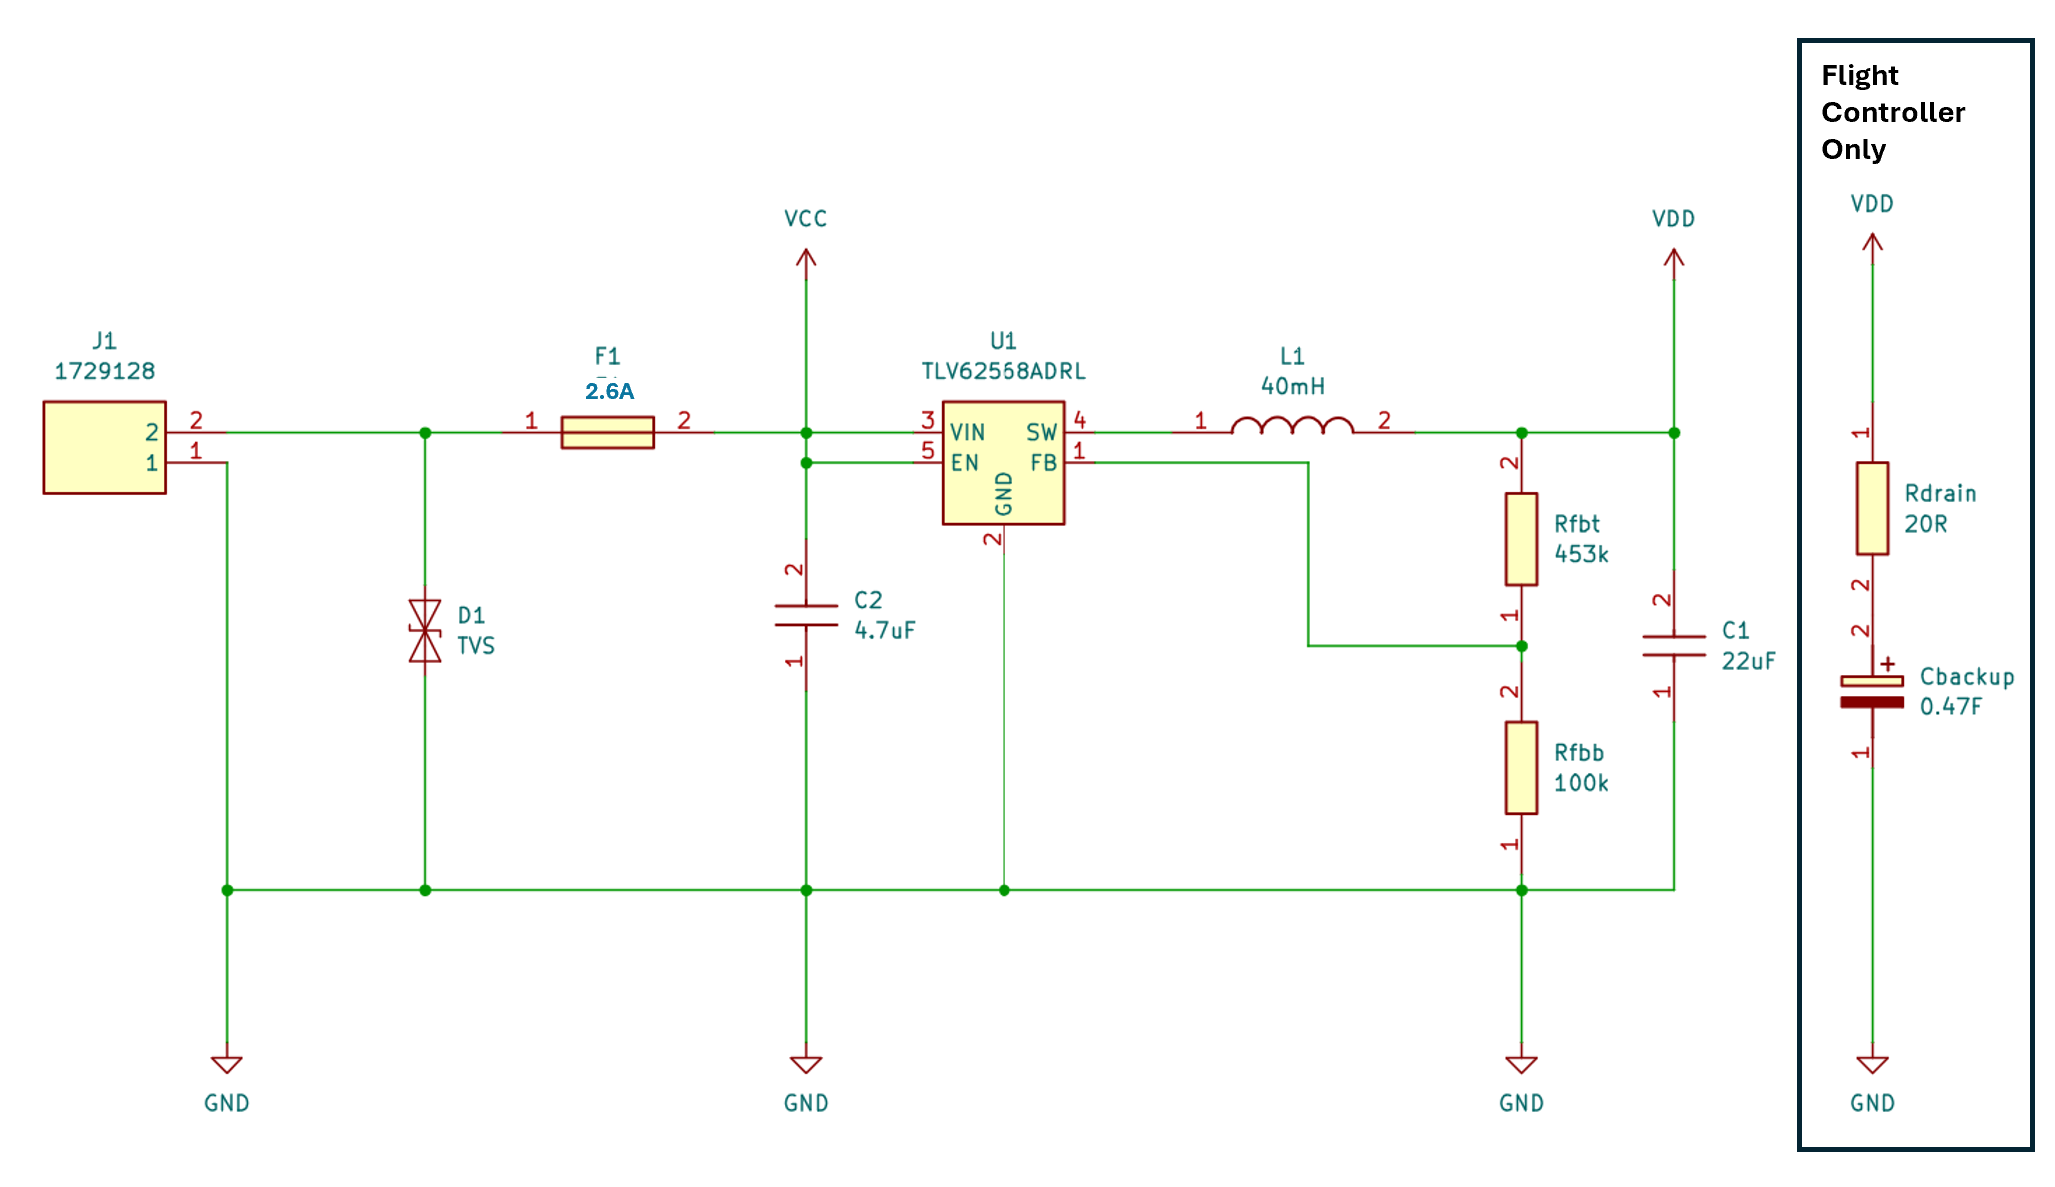
\includegraphics[width=\textwidth]{figs/Thomas/Custom Hardware/Power Supply.png}
  \caption{Power Supply Schematic}
  \label{fig:power_supply_schematic}
\end{figure}



\begin{figure}[htbp]
  \centering
  \begin{subfigure}[b]{0.48\textwidth}
    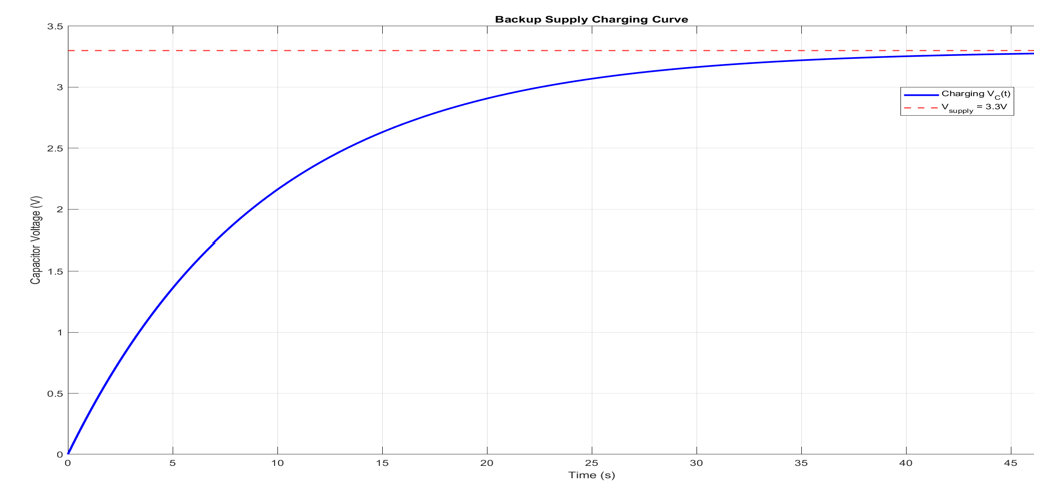
\includegraphics[width=\textwidth]{figs/Thomas/Custom Hardware/charging_curve.png}
    \caption{Backup Power Supply Charging Curve}
    \label{fig:charging_curve}
  \end{subfigure}
  \hfill
  \begin{subfigure}[b]{0.48\textwidth}
    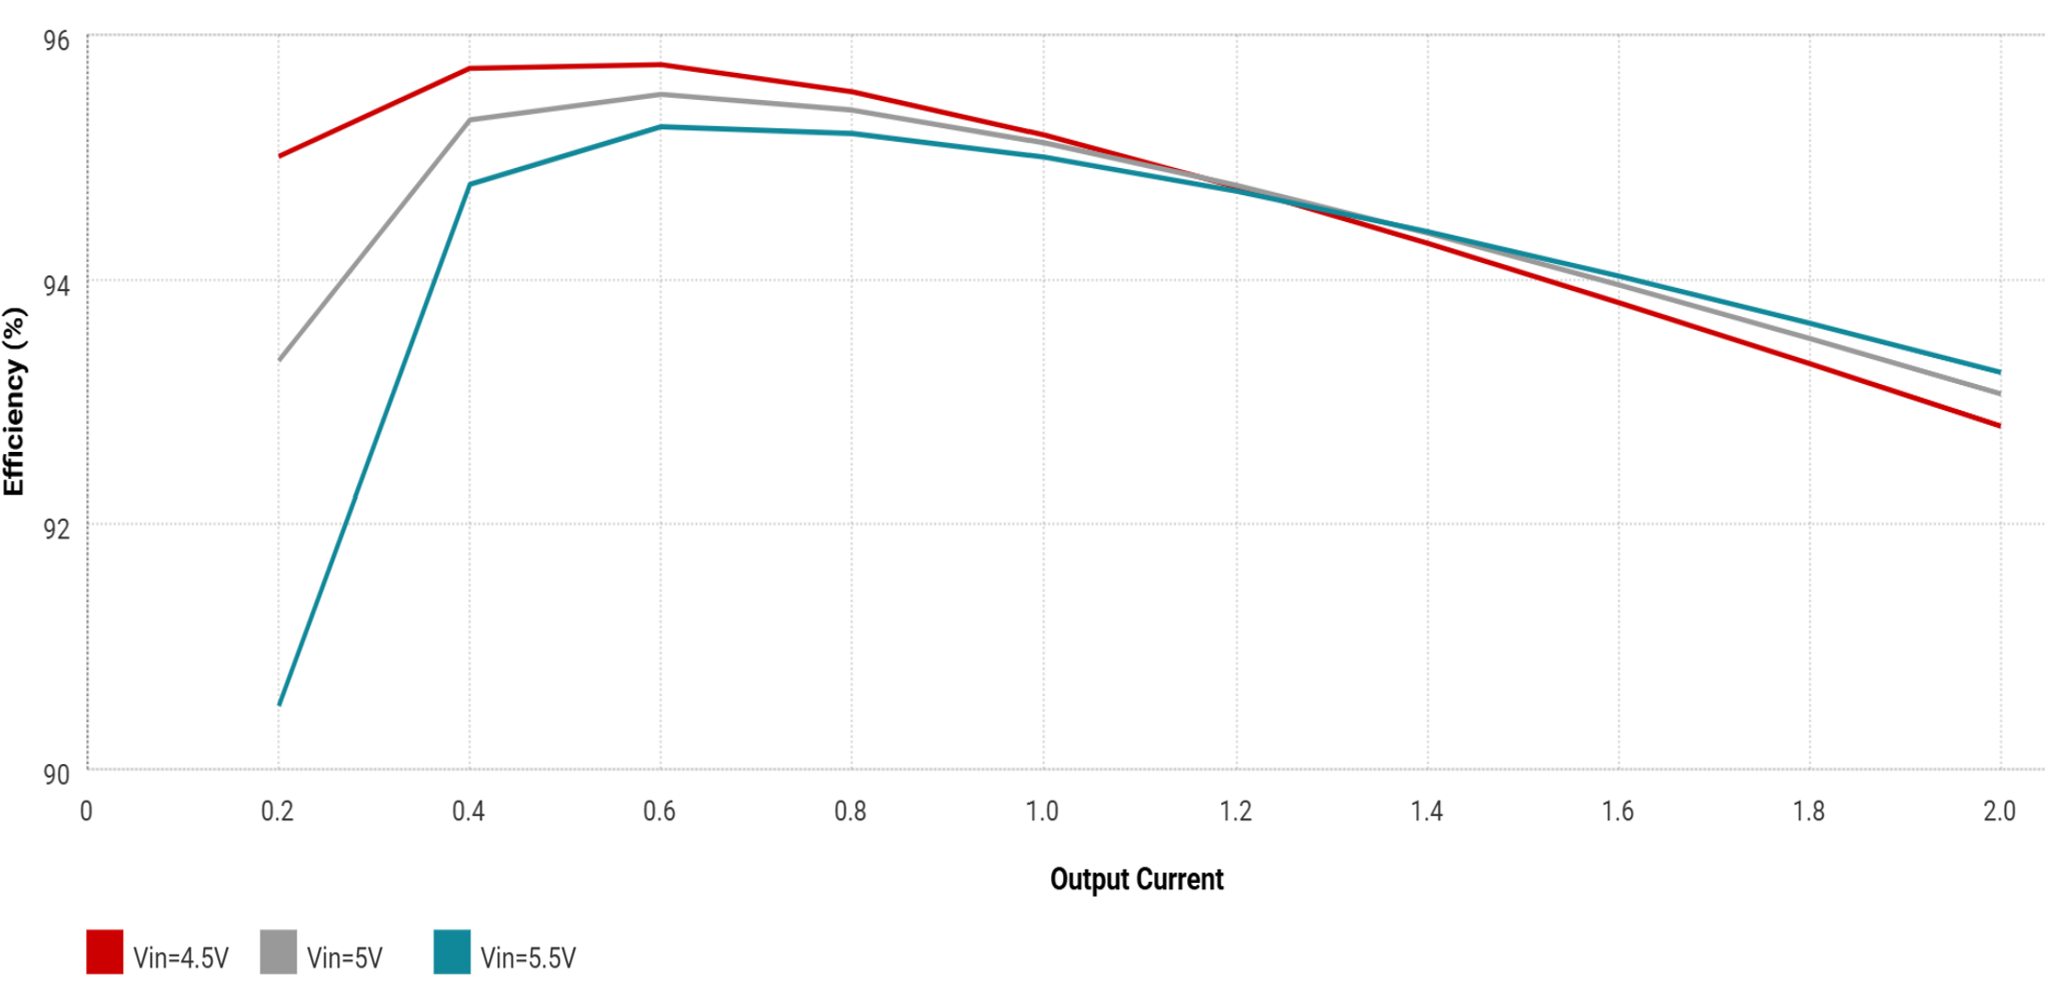
\includegraphics[width=\textwidth]{figs/Thomas/Custom Hardware/Power Module Effciency.png}
    \caption{Power Module Efficiency}
    \label{fig:power_efficiency}
  \end{subfigure}
  \caption{Custom Power Supply}
  \label{fig:power_graphs}
\end{figure}

\paragraph{Backup Power Supply}
The telemetry recordings of the flight controller are vital for crash analysis. However, in cases of sudden electrical failure the data recording will stop before writing the final state vectors and error codes. For example, if before a short circuit the current draw from an \gls{ESC} starts spiking that message needs to be recorded even if a fuse immediately burns shutting down the power supply. Therefore, a supercapacitor in series with a drain resistor is used \ref{fig:power_supply_schematic}. The capacitor selected is rated up to 5.4V at 0.47F\footnote{\url{https://uk.rs-online.com/web/p/supercapacitors/2506967}}. 
\begin{equation}
t = \frac{C \cdot (V_0 - V_{\text{cutoff}})}{I}
\label{eq:discharge_time}
\end{equation}
\begin{equation}
t_{\text{worst-case}} = \frac{0.47 \cdot (3.3 - 2.8)}{1} = 0.235\ \text{seconds}
\label{eq:worst_case_time}
\end{equation}
\begin{equation}
\tau = R \cdot C = 20 \cdot 0.47 = 9.4\ \text{seconds}
\label{eq:charging_time_constant}
\end{equation}
The time before dropout, with the worst case conditions is over 0.2 seconds \ref{eq:worst_case_time}, this will provide sufficient time to record any last messages. Furthermore, the time constant is 9.4s \ref{eq:charging_time_constant} meaning that there are current spikes when turning the device on but it is still charged over 3V within 30 seconds \ref{fig:charging_curve}.

\subsubsection{Comparison to Commercial Options}\label{sub_sub_section:tgt_commercial_options}
\begin{table}[htbp]
  \centering
  \begin{tabular}{|l|r|r|}
    \hline
    \textbf{Category}         & \textbf{Redundant GNSS Cost} & \textbf{Flight Controller Cost}\\ 
    \hline
    Passive Components        & £140.40  & £385.00\\
    Active Components         & £1699.10 & £1865.10\\
    Headers/Connectors        & £179.50  & £278.40\\
    PCB \& Assembly           & £262.14  & £334.04\\
    \hline
    \textbf{Total}            & £2281.14 & £2862.54\\
    \hline
  \end{tabular}
  \caption{Cost of custom component (100 units)}
  \label{tab:aggregated-cost}
\end{table}
The CUAV X7+\footnote{\url{https://store.cuav.net/shop/x7/}} GPS compatible option costs £339.75 and provides the same core functionality as the custom flight controller including dual \gls{CAN} ports. This can be combined with the flight controller compatible with the CUAV C-RTK 9Ps Positioning Module\footnote{\url{https://store.cuav.net/shop/c-rtk-9ps/}} that costs £332.91 for a drone-base station pair and provides \gls{RTK} \gls{GNSS}. This is a significant increase in cost however, it would not require development and may be a superior option in the testing phase. However, for deployment the custom components should be used given the cost implications and that the custom \gls{GNSS} module is fully control capable and the commercial option is not. 


%\newpage
\fancyhead[C]{Rory Millard}
\section{Project Financing} \label{financing}

% --- Introduction: Clearer statement of purpose ---
This section presents an economic analysis comparing the drone-based landmine detection system proposed in this report with legacy manual metal-detector methods, focusing on the cost-effectiveness for surveying \textbf{and demining} operations near Kharkiv, Ukraine. The metric for comparison is the total cost to survey and clear one square kilometre (km²) of land, to a recall of over 90\%. The analysis links the system's financial improvement over the legacy system with sensor performance metrics $P_{sys}$ and $R_{sys}$.


\subsection{Cost Comparison} \label{subsec:cost_structures}

The capital costs of the drone-based system proposed in this report are higher than that of legacy manual techniques, which don't rely on expensive equipment, except from transportation and metal detectors. However, for each system, the operational costs are significantly higher than the upfront capital costs due to the labour intensive surveying and clearance stages. Therefore, to compare the two systems financially, only the operational costs need to be compared, as the capital costs are small in comparison. Operational costs especially dominate if the system is leased out instead of purchased.

Legacy demining operations involve a technical survey phase costing $C_\text{legacy survey} = \$305,000 \text{ per km}^2$ surveyed, followed by a clearance phase with a nominal cost of $C_\text{clearance} = \$2,940,000 \text{ per km}^2$ cleared, according to a report from the Kyiv School of Economics\footnote{\url{https://kse.ua/wp-content/uploads/2023/09/Mining-brief_Final-1.pdf}}. Manual technical surveys typically result in clearing approximately 50\% of the surveyed area, representing a precision improvement of 2$\times$ over indiscriminate 'blind' clearance. This is significantly lower than the 27.7$\times$ estimated for the proposed system in Section \ref{fusion_bounds}. The operational cost of technical survey and clearance for legacy manual methods is estimated as:
\begin{equation}
C_{\text{legacy}} = C_{\text{legacy survey}} + (0.5 \times C_{\text{clearance}}) = \$305,000 + (0.5 \times \$2,940,000) = \$1,775,000 \text{/km}^2 
\end{equation}
The operational cost associated with surveying using the proposed drone-based system needs to be estimated. Operation involves one person working 7 hours per day, which is the high thermal contrast window detailed in Section \ref{compvis_thermalsims}. The thermal drone's scanning rate is 62 m$^2$ every 5 seconds (Section \ref{thermal_selection}). Assuming radar scans can be performed approximately concurrently, the survey duration for 1 km$^2$ is estimated at $\approx$ 4 days. With an operator wage of \$15/hr, the labour cost amounts to approximately \$500/km$^2$. The cost of electricity for battery charging is considered negligible in comparison. The expected system wear and tear must also be factored in, as it represents a large operational cost. This is difficult to quantify precisely without field trials, but the cost is estimated at \$1000/km$^2$. Consequently, the total estimated operational survey cost for the drone-based system is approximately \$1500/km$^2$.

To compare the drone system with legacy methods, the cost of clearing a flagged region is assumed to depend only on the region's area. The total operational cost for the drone system $C_{\text{drone}}$, is therefore determined by the number of flagged points, which is a function of $P_\text{sys}$ and $R_\text{sys}$, as described in Section \ref{subsec:performance_savings}. Table \ref{tab:cost_comparison_structured} presents a comparison of the estimated \textbf{operational} costs.

\begin{table}[h!]
% Removed \small command
\centering
\caption[Operational Cost Comparison]{Operational Cost Comparison: Single Drone-Based System vs. Single Manual Deminer in Kharkiv, Ukraine}
\label{tab:cost_comparison_structured}
\begin{tabular}{lcc} 
\toprule
\textbf{Cost Description} & \textbf{Drone System} & \textbf{Legacy System} \\
\midrule
\multicolumn{3}{l}{}\\
Technical Survey Cost (/km²) & \$1500 & \$305,000 \\ 
Time for Technical Survey (days/km²) &  4 & 2500 \tablefootnote{\url{https://apopo.org/what-we-do/detecting-landmines-and-explosives/how-we-do-it/mine-clearance/}} \\ 
Fraction Flagged for Clearance & 3.6\% & 50\% \\ 
Cost of Clearance (/km²) & \$106,137 & \$1,470,000 \\
 \addlinespace
\textbf{Total Cost to Demine 1 km² } & \textbf{\$107,637} & \textbf{\$1,775,000}  \\
\bottomrule
\end{tabular}
\end{table}

\subsection{Financials of System Performance} \label{subsec:performance_savings}

The operational cost of the proposed system depends on the number of point flagged for mine clearance. This depends on the initial mine density $\rho_0$, and the system's precision $P_{sys}$ and recall $R_{sys}$. The fraction of land flagged for mine clearance ($A_\text{flagged}$) is:
\begin{equation}
A_{\text{flagged}} = \frac{\text{Area Flagged}}{\text{Total Area}} \approx  \frac{\rho_0 R_\text{sys}}{P_\text{sys}}. 
\label{eq:flags_fraction} % Renamed label for clarity
\end{equation}
Given the assumption that the clearance cost just depends on the size of the flagged area, the total operational cost for the drone system per km² ($C_{\text{drone}}$) is:
\begin{equation}
C_{\text{drone}}(P_\text{sys}, R_\text{sys}) = C_{\text{survey}} + A_{\text{flagged}} \times C_{\text{clearance}} 
\approx \$1480 + \left( \frac{\rho_0 R_\text{sys}}{P_\text{sys}} \right) \times \$2,940,000 
\label{eq:drone_op_cost} % New label
\end{equation}



Equation \ref{eq:drone_op_cost} demonstrates that improving $P_{sys}$ results in a large operational cost reduction by reducing the number of points flagged for mine removal. While maximizing recall $R_{sys}$ is important for safety (as discussed in Section \ref{lossmatrix}), achieving high precision is the only way the system can be economically viable. The cost savings by choosing the proposed system over legacy systems are plotted in Figure \ref{fig:financial_savings} as a function of $P_\text{sys}$ and $R_\text{sys}$. The expected region of system performance is also plotted (using the bounds from Section \ref{fusion_bounds}), indicating an \textbf{expected operational cost saving of between $\approx$ \$1.65~m - \$1.75~m per km²} surveyed, over the legacy operational cost of \$1.775~m/km². 


% --- Figure - Needs updated caption reflecting source of data/need for recalc ---
\begin{figure}[h!]
\centering
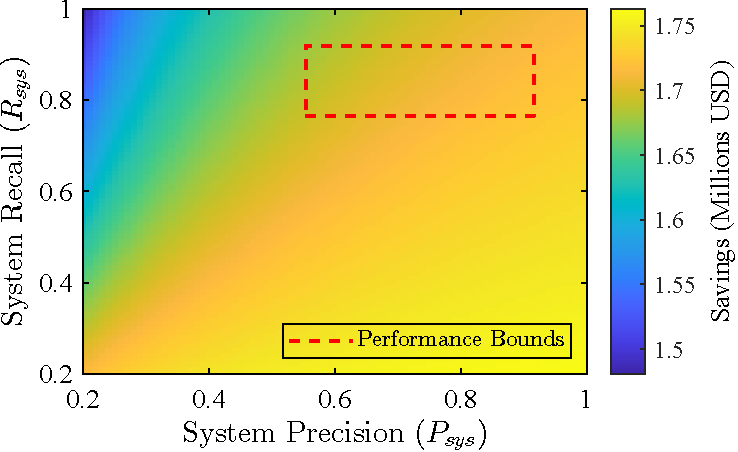
\includegraphics[width=0.5\textwidth]{figs/Rory/financial_savings.pdf} 
\caption[Operational Cost Savings as a Function of Computer Vision Performance]{Plot of Equation \ref{eq:drone_op_cost}. Operational cost savings of the proposed system over legacy systems for surveying and demining 1~km$^2$, varying with $P_{sys}$ and $R_{sys}$. The expected system performance from Section \ref{fusion_bounds} is the region inside the dashed rectangle.}
\label{fig:financial_savings}
\end{figure}


\subsection{Conclusion} \label{subsec:finance_conclusion}

This section strongly suggests that the drone-based detection system proposed in this report offers significant financial benefits over legacy manual demining techniques. The operational costs are reduced by a factor of over 20$\times$, whilst the system is significantly faster. The improved precision means that the area flagged for clearance is much smaller than in legacy techniques, which causes a large reduction in the most significant part of the operational costs and times. These reductions in cost and time will enable more widespread demining operations, restoring large areas of productive land, and saving countless lives. 

Future work should investigate more accurate cost estimates. For the operational costs, more advanced YOLOv11 models (Section \ref{compvis_implementation}) should be trained on real world experimental data. The ANFIS network (Section \ref{fusion}) should be implemented, and the performance metrics $P_\text{sys}$ and $R_\text{sys}$ should be found by testing the entire system on a large dataset of unseen experimental data. This would give a more accurate picture of the system's financial viability, which would help in securing funding if the project were commercialised.



\fancyhead[C]{Student}
\printbibliography{biblio}

% Appendix
% Essential content that interrupts the flow of the document can be placed here, e.g. technical drawings, detailed lists of equations used, etc.
\newpage
\addcontentsline{toc}{section}{Appendix}
\section*{Appendix}

\end{document}
